\documentclass{book}

\usepackage[dvipsnames]{xcolor}
\usepackage{ctex}
\usepackage{amsmath}
\usepackage{amssymb}
\usepackage{physics}
\usepackage{graphicx}
\usepackage{listings}
\usepackage{chemformula}


\usepackage{minitoc} % 每一部分前生成标题

\usepackage{imakeidx} % 创建索引表

% 着重号
\usepackage{xeCJKfntef}
% \xeCJKsetup{underdot/symbol={\normalfont^^b7}}
% \newcommand{\dotemph}[1]{\CJKunderdot{#1}}

% ----------取消注释以调整页边距-----------
% \usepackage{geometry} % 页边距
% \geometry{a4paper,left=2.54cm,right=2.54cm,top=3.18cm,bottom=3.18cm}
% ------------------------------------

% 设置代码块样式
\lstset{
numbersep=1.5em, % 设置语言
 basicstyle=\ttfamily, % 设置字体族
 breaklines=true, % 自动换行
 keywordstyle=\bfseries\color{blue}, % 设置关键字为粗体,颜色为 NavyBlue
 morekeywords={}, % 设置更多的关键字,用逗号分隔
 emph={self}, % 指定强调词,如果有多个,用逗号隔开
    emphstyle=\bfseries\color{Rhodamine}, % 强调词样式设置
    commentstyle=\itshape\color{black!50!white}, % 设置注释样式,斜体,浅灰色
    stringstyle=\bfseries\color{PineGreen!90!black}, % 设置字符串样式
    columns=flexible,
    frame=shadowbox, % 边框
    rulesepcolor=\color{red!20!green!20!blue!20},
    framesep=1em % 设置代码与边框的距离
}

\setcounter{tocdepth}{0} % 目录显示到章

\newcommand{\keyword}[1]{\texttt{#1}\index{#1}}
\newcommand{\keywordin}[2]{\texttt{#2}\index{#1!#2}}
\newcommand{\code}[1]{\texttt{#1}}
\renewcommand{\emph}[1]{\CJKunderdot{\textbf{#1}}}

\newenvironment{Abstract}{在本节,你将要学到:\begin{itemize}}{\end{itemize}}
% \newenvironment{attention}{\begin{center}**********以下内容为注意**********\end{center}\itshape 注意:}{\begin{center}**********以上内容为注意**********\end{center}}
\newenvironment{attention}{\color{red}\itshape 注意:}{}
\newenvironment{extend}{\color{gray}\itshape 补充:}{}
\newcommand{\sectionAuthor}[1]{本节作者:#1\\}
\newcommand{\answer}[1]{\rotatebox{180}{【答案】:#1}\vspace{2em}}
\newcommand{\texttilde}{\textasciitilde}
\newcommand{\ttilde}{\texttilde}

\bibliographystyle{unsrt} % 参考文献样式

\title{针对VASP的材料计算教程\\为材料计算而生}

\author{Jiaqi Z.\footnote{Copyright © 2024 Jiaqi Z. All rights reserved.}}

\makeindex

\begin{document}

    \maketitle

    \frontmatter

    \dominitoc

    \tableofcontents

    \include{preface/前言}

    \include{temp.tex}

    \mainmatter

    \part{Linux基础}

    \input{Linux基础/Linux命令行操作/Linux命令行操作.tex}
\input{Linux基础/文本编辑工具vi和vim/文本编辑工具vi和vim.tex}
\chapter{高级Linux命令}\label{chap:高级Linux命令}
\minitoc

\input{Linux基础/高级Linux命令/通配符/通配符.tex}
\input{Linux基础/高级Linux命令/grep匹配字符串/grep匹配字符串.tex}
% 请在下方的大括号相应位置填写正确的节标题和标签,以及作者姓名
\section{sed文本替换}\label{sec:sed文本替换}
\sectionAuthor{Jiaqi Z.}

% 请在下方的item内填写本节知识点
\begin{Abstract}
    \item 如何使用\code{sed}命令对文本文件进行替换
    \item 如何使用\code{sed}查看文件内容
    \item 如何使用\code{sed}添加(删除)文本文件的内容
\end{Abstract}

% 请在正文相应位置填写正确的小节标题(或小小节标题),同时将标签的“节标题”和“小节标题”改为实际内容

在\ref{sec:查找与替换}当中,已经介绍了如何使用vim进行文本文件的替换。与vi里面的\code{s}命令类似,在命令行也有类似的方式可以对文本文件进行替换(甚至更复杂的操作)。那就是使用\keyword{sed}命令。

\subsection{使用\code{sed}显示}\label{subsec:sed文本替换-使用sed显示}

\code{sed}的语法格式是:\code{sed [选项] "<动作>" [文件路径]}。其中,常见的选项包括

\begin{itemize}
    \item \keywordin{sed}{-n} 表示\emph{只有处理的文本}显示在屏幕上(默认是全部文本)
    \item \keywordin{sed}{-i} 表示\emph{直接修改文件内容}。
\end{itemize}

\begin{attention}
    在本节,我们所处理的文件都会使用\code{-i}选项直接对文件进行处理。但这一行为是危险的,尤其是对于不确定的修改操作,由于它是对原文件进行修改,因此需要提前备份。此外,千万不要将\code{-n}和\code{-i}结合起来使用,它表示\emph{仅将处理的文本修改为文件内容}。

    在下一节将介绍管道运算符和重定向运算符,将会帮助你避免这一问题。
\end{attention}

\begin{extend}
    如果你仔细观察上面的语法格式,需要特别注意的是里面的\code{[文件路径]}是“可选”的,也就是说,\emph{对于\code{sed}命令而言,可以不提供文件路径}。这件事可能会比较“难以置信”,毕竟如果没有文件,怎样处理文件呢?

    事实上,\code{sed}命令是一个\emph{管道命令},简单来说,它是可以读取并处理终端输出的内容。除此之外,像前面的\code{grep}也是类似的(虽然我们前面并没有特别强调这一点)。

    在下一节,我们将详细讨论管道命令的内容。
\end{extend}

让我们先来看一个最简单的操作——\emph{打印},即试着将特定几行的内容打印在屏幕上。其在“动作”部分的写法是\code{<开始行号>,<结束行号>p}。例如,我们希望将\code{POSCAR}的第3-5行输出,可以使用命令\code{sed -n "3,5p" POSCAR}表示输出第3-5行内容。

\begin{extend}
    如果你此时忘记了\code{-n}选项的话,命令将会输出所有的\code{POSCAR}文件,但对应行号的内容会重复输出。(可以试试)

    另外,如果希望对最后一行进行操作,需要使用\code{\$}符号表示\emph{最后一行},但此时\emph{需要将外面的双引号变为单引号}。通常情况下,双引号和单引号是等价的,但在涉及到\code{\$}符号时,使用双引号则表示将\code{\$}和后面的符号(例如\code{\$p})解析成\emph{变量p},而使用单引号则表明这一符号就是符号本身。变量的作用,将在后面循环和批量处理中体现,在此不做讨论。
\end{extend}

\subsection{使用\code{sed}添加和删除}\label{subsec:sed文本替换-使用sed添加和删除}

使用\code{sed}命令删除某一行的方法是使用\code{d},例如,如果希望删除\code{POSCAR}文件的第3-5行,类似于上面的显示,使用方法是\code{sed -n "3,5d" POSCAR}

\begin{attention}
    这一操作是对文件内容进行删除,因此你应该谨慎使用\code{-i}选项(会直接将原文件对应内容删除),在下一节的重定向运算符将会提供灵活的解决方法。目前的一个方法是\emph{创建一个备份文件}。
\end{attention}

对于添加某行内容,可以使用\code{a}或\code{i},前者表示\emph{新增(在下一行)},后者表示\emph{插入(在上一行)}。具体的,其命令为:\code{sed [选项] "行号a(i) 添加字符串" [文件名]}例如,希望在\code{POSCAR}的第一行后面添加一个字符串“1.0”,可以使用\code{sed -n "1a 1.0" POSCAR}。

那么,如果希望在第一行添加内容,应当怎么办呢?

\answer{\code{sed -n "1i 1.0" POSCAR}即可。}

\subsection{使用\code{sed}替换}\label{subsec:sed文本替换-使用sed替换}

使用\code{sed}替换有两种模式,分别是\emph{整行替换}和\emph{字符串替换}。对于整行替换,命令为\code{sed [选项] "行号c 替换目标字符串" [文件名]}。例如,若希望将\code{POSCAR}的第2行替换为“0.8”,则可以使用命令:\code{sed -n "2c 0.8" POSCAR}。

相比于整行替换,字符串替换可能更为强大。与vim的替换类似,在\code{sed}当中替换字符串的命令是\code{sed [选项] "s/要被替换的字符串/新字符串/g"}。例如,希望在\code{INCAR}当中的\code{ENCUT=400}替换为\code{ENCUT=600},可以使用命令\code{sed "s/ENCUT=400/ENCUT=600/g" INCAR}。

对于字符串替换而言,更重要的是\emph{支持正则表达式}(关于正则表达式的内容详见\ref{sec:初窥正则表达式}一节),例如,在上面的例子中,我们希望将\code{ENCUT=400}或\code{ENCUT=600}全部替换为\code{ENCUT=800},则可以使用\code{sed "s/ENCUT=$\backslash$ d$\backslash$ d$\backslash$ d/ENCUT=800/g" INCAR}

\begin{attention}
    同样,由于这是对内容的删除(更改),因此需要提前备份。除非有足够的把握,否则不要使用\code{-i}选项。
\end{attention}


\subsection{错误处理}\label{subsec:sed文本替换-错误处理}
% 请在本节列出可能遇见的错误与解决方法

\subsubsection{sed: -e expression \#1, char 2: invalid usage of line address 0}

在使用行号时,第一行是1而不是0. 通常来说,当你试图在第1行插入数据时,应当使用\code{sed -n "1i 字符串" [文件名]},其中\code{i}表示在第1行前面插入数据(即在第一行写入字符串)
% 请在下方的大括号相应位置填写正确的节标题和标签,以及作者姓名
\section{管道与重定向}\label{sec:管道与重定向}
\sectionAuthor{Jiaqi Z.}

% 请在下方的item内填写本节知识点
\begin{Abstract}
    \item 管道运算符、如何使用管道运算符连接多个命令
    \item 使用重定向写入(读取)文本文件
\end{Abstract}

% 请在正文相应位置填写正确的小节标题(或小小节标题),同时将标签的“节标题”和“小节标题”改为实际内容

\subsection{管道}\label{subsec:管道与重定向-管道}

在\ref{sec:sed文本替换}一节当中,我们讨论了如何使用\code{sed}命令对文本文件进行编辑。当时我们提到,\code{sed}命令是一个管道命令,可以读取终端输出的内容。除此之外,在很多时候我们希望对某一文件进行多次操作,例如,提取某一文件的前10行,并将其中的“C”改成“B”,然后再写入新的文件当中。

像上面这种输入和输出层层传递的(一个命令的输出作为另一个命令的输入),就可以使用这一节的“管道”命令。在Linux当中,管道运算符是\code{|}(通常是Shift+Backspace下面的那个键),它的作用是\emph{把前面命令的输出作为下一个命令的参数输入}。例如,我们希望将\code{POSCAR}输出,可以使用\code{cat POSCAR},若此时又想取出前5行,则可以使用\code{cat POSCAR | head -n 5}

\begin{attention}
    也许使用\code{head -n 5 POSCAR}一样可以解决上述问题,但使用管道更具有“可扩展性”。例如,\code{cat}命令本意是将多个文件连接起来,若希望将连接之后的文件读取前5行,则使用管道运算符是最简单的方法之一。
\end{attention}

上面的过程,可以看作是将\code{cat}命令输出结果作为\code{head}命令的参数输入,之后运行\code{head}命令并输出(至标准输出),进一步,如果我们希望将其中的“C”全部替换成“B”,则需要借助于\code{sed}命令,表示为:\code{cat POSCAR | head -n 5 | sed "s/C/B/g"}

\begin{attention}
    此时使用\code{sed}命令由于没有添加\code{-i}选项,因此结果也仅仅在标准输出当中进行输出,源文件并没有修改。
\end{attention}

类似地,如果我们希望得到\code{OUTCAR}最后一个包含“without”字符串的行,在使用管道之前是“几乎不可能”的,而在利用管道时,便可以使用命令:\code{grep without OUTCAR | tail -n 1}得到结果\footnote{这一过程实际上是在VASP当中得到最后收敛能量的过程。}。

\subsection{输出重定向与输入重定向}\label{subsec:管道与重定向-输出重定向与输入重定向}

在之前,我们得到的输出结果仅仅是在屏幕上输出(也被称为“标准输出”),但必要的时候,我们也希望将结果保存至本地,以便后续处理(无论是进一步使用程序语言读取并处理,还是过一段时间再看)。正因如此,寻找一种方法将输出结果保存就十分重要。

在Linux当中,保存终端输出的本质就是“将输出\emph{重定向}至文件”,其运算符是\code{>}或\code{>>},后面需要有一个文件名路径表示\emph{希望写入的文件}。其中,前者(\code{>})表示\emph{创建},当文件存在时则会覆盖;后者(\code{>>})表示\emph{追加},当文件不存在时新建,存在时则会在后面追加新的内容。

有了这一方法,我们终于可以解决\ref{sec:sed文本替换}一节所遗留的关键问题:如何将编辑后的文件保存至新的文件?答案就是\emph{使用重定向运算符}。例如,我们希望将\code{INCAR}文件里面的\code{ENCUT=400}改为\code{ENCUT=600}并保存至\code{INCAR2},则可以使用命令:\code{sed "s/ENCUT=400/ENCUT=600/g" INCAR > INCAR2}

再一个例子,如果希望将\code{Si/POTCAR}和\code{O/POTCAR}合并至一个新的\code{POTCAR}当中,应当怎样写呢?

\answer{\code{cat Si/POTCAR O/POTCAR > POTCAR}}

\begin{extend}
    请注意运算符是\code{>}而不是\code{<},前者表示“输出重定向”,而后者表示“输入重定向”,即将文件的内容作为命令的输入。例如,\code{cat < POSCAR}与\code{cat POSCAR}等价。

    二者的方向虽然容易混淆,但似乎可以从箭头的方向看出一点规律——\code{>}表示将命令的内容“输出至”文件中,而\code{<}表示将文件“输入至”命令中。
\end{extend}

在必要的时候,我们当然也可以将输入和输出同时重定向,例如,\code{cat < POSCAR > POSCAR2}也是可行的(将\code{POSCAR}重定向输入至\code{cat}命令,并将命令输出结果重定向至\code{POSCAR2}输出)

\begin{extend}
    除了“标准输入”和“标准输出”之外,Linux还有一个“标准错误输出”,用来输出命令运行报错的结果。例如,当我们希望删除一个名为\code{POSCUT}的文件时(该文件并不存在),使用\code{rm POSCUT}会报错(这一点在\ref{sec:文件操作}已经详细讨论过了)。如果试图将这一输出重定向,例如,\code{rm POSCUT > output},效果是一样的。但如果使用\code{rm POSCUT 2> output}呢?你会发现,终端没有报错了,而将报错输出至文件\code{outcar}当中了。这其中,\code{2>}就表示将“标准错误输出”重定向至后面的文件。

    在这一基础上,稍微扩展一下。在后面的VASP教程中,我们将看到提交脚本中有\code{mpirun vasp\_std > vasp.out 2>vasp.err}这一行\footnote{不同课题组可能有所不同,这里仅仅作为例子。}。暂且忽略掉前面的\code{mpirun}(表示分布式计算系统下并行运行任务),可以发现,这一行的作用就是运行\code{vasp\_std},并将输出结果输出至\code{vasp.out},而将错误信息输出至\code{vasp.err}。

    另外,我们这里重定向的文件并不一定是文本文件。如果你回顾一下\ref{subsec:查看文件-Linux文件类型}一节,可能会发现里面有一个“设备文件”,它也是可以作为重定向输入输出的一部分。例如,\code{rm POSCUT 2> /dev/null}则表示将输出报错信息重定向至\code{/dev/null}设备(这是一个“空设备”,用于消除所输出的内容)。运行这一命令,你将不会得到任何输出结果(输出被消除了)
\end{extend}


\subsection{错误处理}\label{subsec:管道与重定向-错误处理}
% 请在本节列出可能遇见的错误与解决方法

\subsubsection{使用\code{cat << POSCAR}没有反应}

如果你确实希望使用输入重定向,应当注意是\code{<}(一个)而不是\code{<<}(两个)。后者在Linux中通常用于终端交互中,例如,上面的命令表示将\code{POSCAR}之间的内容作为输入。一个演示例子为:

\begin{lstlisting}[language=bash]
$ cat << POSCAR
> hello
> world
> POSCAR
hello
world
\end{lstlisting}

可以看到,它把“POSCAR”之间的内容传入了\code{cat}命令(输出)



\chapter{Shell脚本基础}\label{chap:Shell脚本基础}
\minitoc

% 请在下方的大括号相应位置填写正确的节标题和标签,以及作者姓名
\section{第一个脚本}\label{sec:第一个脚本}
\sectionAuthor{Jiaqi Z.}

\begin{Abstract}
    \item 什么是Shell脚本
    \item 如何编写第一个Shell脚本——Hello World
    \item 如何运行脚本
\end{Abstract}

在前面的学习中,我们已经了解如何使用Linux命令在Shell进行操作,我们了解了如何对文件和目录进行简单的操作(如删除、复制等),同时我们也了解了一些更复杂的操作,例如使用\code{grep}和\code{sed}进行文本的查找和替换等。最后,我们还了解了如何使用\code{for}循环来进行批量操作。

而在一些特殊的场景下,我们可能希望做更复杂的操作,或者说,我们希望更简单地执行一些操作(这两句话本质上是一样的)。例如,如果我们每次都需要使用\code{sed}命令修改特定的内容,如\code{ENCUT = 400},刚开始还好,时间长了可能就会“嫌麻烦”。此时可能就会希望有一个单独的命令(比如叫做\code{changeENCUT})来实现这一功能。而实现这一功能的方法,就是使用\emph{脚本}。

在本章,我们将会讨论如何编写自己的脚本。类似于编程语言,脚本里面将会包含大量的编程思想——如输入、输出、条件、判断、函数等。在学习这一部分之前,希望你已经有了部分编程语言基础(没有也没有关系)。

\begin{extend}
    关于Shell和Bash的区别:一般来说,Shell指的是系统和用户交互的那层“外壳”,之前我们所学习的内容,其操作都是在Shell当中进行的。Shell具有多种版本,如“Bourne Shell”、“Bourne Again Shell”、“C Shell”等。其中,“Bourne Again Shell”就是我们所谓的“bash”。在你的操作系统下,可以使用\code{top}命令查看其Shell类型。
    
    Shell脚本,全称叫做“Shell Script”,是一种在Shell当中批量运行多条语句的程序。
    
    由于目前主流的Shell是基于Bash解释的,而我们所写的Shell脚本,实际上也大多都是Bash脚本,因此在后文当中,我们可能不会精确区分Bash脚本和Shell脚本的区别。
\end{extend}

\subsection{编写第一个脚本}\label{subsec:第一个脚本-编写第一个脚本}

正如任何程序的开始都是“Hello World”,在本章我们也不例外。在Linux当中编写Shell脚本不需要额外的程序,只需要使用\code{vi}编写一段文本文件,并\emph{赋予它运行权限},就可以作为脚本运行了。首先通过\code{vi}创建一个名为\code{hello}的文件,并输入如下内容:

\begin{lstlisting}[language=bash,label=hello]
#!/bin/bash
# 输出Hello World!
echo "Hello World!"
\end{lstlisting}

编写完成后保存,并添加运行权限(\code{chmod +x hello},详见第\ref{sec:文件权限管理}一节),然后执行\code{./hello},即可在屏幕上看到输出结果。

\begin{attention}
    在运行时需要加上\code{./}表示在当前目录寻找命令。在Linux当中,不添加\code{./}表示在环境变量\code{PATH}下查找文件运行,你可以在家目录下找到\code{.bashrc}的文件,里面包含有一系列配置Bash的命令,其中就有对环境变量的设置。

    在运行前,你需要保证程序已经具有运行权限,或者可以使用\code{source ./hello}或\code{. ./hello}的方式(二者等价)“临时赋予运行权限”\footnote{这是表面上的用法,事实上,\keyword{source}本意是\emph{在当前Shell下运行文件}。相对的,其他的用法(不加\code{source})则是在当前shell下新建了一个“子Shell”运行代码,其运行结果(例如一些变量)并不会带回外面。}。
\end{attention}

其中,代码第一行\code{\#!/bin/bash}表示\emph{使用bash运行}。正如前面所说的那样,Shell具有多种版本,因此,在编写时应当特别指定你所使用的版本。由于目前大多数Shell都是使用Bash,因此这一行在有些时候“可以省略”。但我们不建议将其省略,因为\emph{你永远不能保证你的这个脚本今后会在哪个版本的Shell下运行}。

\begin{extend}
    你可以想见,\code{/bin/bash}就是\code{bash}命令所在位置,你可以去看一下是不是真的存在。在查看的时候,注意是从“根目录”开始而不是“家目录”

    如果你真的这么做了,一种简单的方法是在\code{/bin/}目录下使用\code{ls | grep bash}只输出具有“bash”的文件,从而简化输出结果。当然,你也可以直接使用\code{ls bash}查看。

    当然,不建议你尝试使用\code{vi bash}查看里面的内容,\emph{它不是文本文件}。
\end{extend}

代码第二行以\code{\#}开头表示\emph{注释}。如同编写其他代码一样,使用注释是一个好习惯,它可以帮助你划分代码段落,以及记住对应的功能。随着学习的深入,我们会编写越来越长的脚本。因此,记得加注释是个好习惯。

第三行是这一脚本的关键,它使用\keyword{echo}实现字符串的输出。事实上,Shell脚本的每一个命令都可以在Shell本身下运行。因此,你也可以直接在Shell运行这一命令,会实现同样的效果。而编写脚本之后,就可以直接通过\code{./hello}实现这一功能,这便是脚本的作用。

\begin{attention}
    \code{echo}会将它后面的所有内容输出(在其他一些编程教材中,会将这一功能叫做“应声虫”,实际上,echo也就是“回音”的意思)。我们在这里添加双引号是为了强调它们是整体的,事实上,当你去掉这两个双引号,对程序运行结果没有任何影响。

    如果你在你的脚本中编写了代码,并同样使用了双引号,请注意:\emph{使用英文符号而不是中文符号},这一点在后续所有脚本编写过程中都应当注意。一般来说,我们不建议在脚本当中添加中文,虽然你写\code{echo "你好,世界!"}可能也会得到正确的结果,但不会永远如此。

    在本章的教程中,为了考虑到读者水平,我们的注释部分都会采用中文,如果这样也会引起脚本运行的失败(在测试时正常,但不敢保证在你的电脑也会正常),请删除中文注释后运行。
\end{attention}

\subsection{添加至环境变量}\label{subsec:第一个脚本-添加至环境变量}

正如前面所说,使用\code{./hello}表示在当前目录下查找名为\code{hello}的脚本并运行。这可以帮助我们快速调试代码,但在真正应用时,我们可能会希望在任何目录下运行脚本。此时就会希望将代码添加至环境变量,也就是前面所说的\code{PATH}。添加方法有两种——将脚本放置到已有的环境变量中,或者将脚本所在的目录设置为环境变量。

你可以通过\code{\$PATH}命令输出当前环境变量,通常来说,你可以将你所编写的脚本命令放置在\code{\texttilde/bin/}目录下(这一般都是用户的环境变量)完成后,你可以在任何目录下运行你的脚本了(不需要\code{./}了)。例如,在完成上述配置后,在任何目录下运行只需要使用\code{hello}即可。

如果你编写了一系列脚本,一个简单的方法是直接将它们所在的目录设置成“环境变量”。此时需要通过\code{.bashrc}文件。假设你的脚本所在目录为\code{\texttilde/bash/},使用\code{vi}打开\code{.bashrc}文件,在最后一行添加\code{export PATH=\$HOME/bash:\$PATH}即可。

其中,\keyword{export}是用来设置“环境变量”的命令,后面的\code{PATH=...}则是“变量赋值”的过程(后面就会学到)。\code{\$HOME}是系统内置的变量,表示\emph{用户的家目录},你可以在Shell下使用\code{echo \$HOME}查看变量的值\footnote{在这里我们又不知不觉接触到\code{echo}的新用法:输出变量的值。这本是后面的内容,在这里你可以提前先了解一下。},后面的\code{\$PATH}则表示原先的环境变量。

简单说,这一语句的意思就是在原有的\code{PATH}变量前面添加一个新的\code{\$HOME/bash}。添加完成后你需要使用\code{source \texttilde/.bashrc}命令“激活”这一环境变量(或者重启也可以实现这一功能),然后即可在任何地方如一般运行命令一样运行你在\code{\texttilde/bash/}目录下所有的脚本了。

\begin{attention}
    在后面的教学演示中,我们都不会添加\code{./}运行脚本(或者说,只有在这一节我们会详细提到如何运行脚本,后面都简单说作“运行脚本”)。如无特殊说明,无论是哪种方法(在当前目录、添加环境变量),运行最终效果都是一样的,后面不再赘述。

    为了你的方便,建议新建一个目录作为你后续练习脚本的目录,并使用上面的方法将其添加到环境变量中。
\end{attention}


\subsection{错误处理}\label{subsec:第一个脚本-错误处理}

\subsubsection{-bash: <脚本名>: Permission denied}

这可能是因为你在运行脚本时没有赋予其运行权限而直接运行脚本,如果你没有赋予权限,请使用\code{source}命令或\code{.}运行脚本。这同样适用于环境变量中的命令。对于环境变量中没有运行权限的脚本,需要使用\code{source <脚本名>}或\code{. <脚本名>}执行。
% 请在下方的大括号相应位置填写正确的节标题和标签,以及作者姓名
\section{变量}\label{sec:变量}
\sectionAuthor{Jiaqi Z.}

% 请在下方的item内填写本节知识点
\begin{Abstract}
    \item 如何在脚本中定义变量
    \item 如何输出变量
    \item 如何对变量进行简单运算
\end{Abstract}

% 请在正文相应位置填写正确的小节标题(或小小节标题),同时将标签的“节标题”和“小节标题”改为实际内容

如果所有脚本都只能按照固定的内容运行,显然功能太弱了。与其他编程语言类似,脚本语言应当也具有类似于“\emph{变量}”的功能实现“可拓展性”。

所谓“变量”,指的就是\emph{在运行过程中会发生变化的量},这些值可能是由用户输入给定的,或者在运行过程中生成的,或者是通过文件读取得到的。

\subsection{定义变量与初始化}\label{subsec:变量-定义变量与初始化}

与C语言等强类型语言不同,Shell脚本的变量在使用之前不需要对其进行“声明”,相对地则是需要对其进行\emph{初始化}。与其他编程语言类似,在Shell脚本中,第一次使用变量时需要对变量进行赋值(也可以叫做“初始化”)。例如,我们希望将字符串“Hello World!”赋值给一个变量,则可以使用\code{STRING="Hello World!"}

\begin{attention}
    与其他编程语言类似,在Shell脚本中,赋值也是使用\code{=}运算符。但不同的一点是,在运算符两侧\emph{不能有空格}。

    在变量命名时,需要遵守如下原则:变量名只能包括数字、字母和下划线(\code{\_}),第一个字符不能是数字,不能是已有的关键字\footnote{“关键字”指的是在Shell脚本中已经具有特定含义的词语,如\code{echo}就不能作为变量名。}。
\end{attention}

在一个程序中,可以同时存在多个变量,对于已经赋值的变量,也可以对其再次进行赋值(原有值会发生变化)。例如,下面的代码:

\begin{lstlisting}[language=bash,caption=variable,numbers=left]
#! /bin/bash
# 变量初始化
STRING1="Hello World!"
STRING2="I Like Bash"
STRING2="I Like Shell Script"
\end{lstlisting}

上述代码第3行定义了一个变量\code{STRING1},其赋值为\code{"Hello World!"};在第4行,首先定义了一个变量叫做\code{STRING2},首先赋值为\code{"I Like Bash"},在第5行又一次对其进行赋值,此时\code{STRING2}的值变为\code{"I Like Shell Script"}。

\subsection{调用变量}\label{subsec:变量-调用变量}

如果你熟悉其他编程语言如C、Java、Python等,也许在编写上面的语句时,你会很自然写出如\code{STRING2=STRING1}这样的语句。在你看来,这好像是把\code{STRING1}的值赋值给\code{STRING2},但当你运行时,发现事实并非如此。这是因为在Shell脚本中,变量的调用需要用到其他的方法。

\begin{attention}
    在上面我们提到\code{STRING2=STRING1}的含义是\emph{将\code{STRING1}的值赋值给\code{STRING2}},这对于了解过其他编程语言的读者而言是很自然的。但如果你没有学习过其他编程语言,需要特别注意的一点是:在程序设计语言中(几乎大多数的程序语言),\code{=}所表示的含义与你所熟悉的数学上的含义不同。在数学上,=表示一种\emph{状态},表达两个值相等;而在程序设计中,\code{=}表示将右边的值\emph{赋值给}左边的值(一种\emph{动作})。

    尽管在最后的结果上,二者是相同的,但数学上的=表达一种“状态”,而程序设计中表达一种“动作”,是不同的。一个很简单的例子就是上面的\code{STRING2=STRING1},从数学的角度看,这显然不成立,因为\code{"I Like Shell Script"}显然不可能\emph{等于}\code{"Hello World!"},但程序设计上是可行的,因为它表达了“赋值”的动作。

    也正因如此,在数学上,$a$和$b$相等写成$a=b$或者$b=a$都是可行的(这也就是等式的“对称性”);而对于程序设计而言,\code{a=b}和\code{b=a}显然是不同的,因为它们所表达的动作“方向”是不同的。
\end{attention}

在Shell脚本中,调用变量需要使用到\keyword{\$}符号。事实上,这不是你第一次见到它(如果你忘记了,请回到\ref{sec:简单for循环}一节,或者更准确的,\ref{subsec:简单for循环-关于变量}一节)。与定义变量不同,在Shell脚本中,但凡是需要\emph{调用变量}的地方,都需要使用\code{\$}符号。例如,在上面的例子中,如果你确实希望表达\code{STRING2=STRING1},需要写作\code{STRING2=\$STRING1}。

这里有一点“小绕”的地方在于,为什么在\code{STRING2}前面不需要添加\code{\$}符号。这是因为,我们实际上只是调用了\code{STRING1}变量的值,并不关心\code{STRING2}里面是\code{"I Like Shell Script"}还是\code{"I Like Roselia"}。因此,我们只需要通过\code{\$STRING1}来获得\code{STRING1}的值。

\begin{extend}
    你还可以做一个“不准确”的理解:\code{\$}总是视图将右边的内容“展开”为完整的内容。例如,假设\code{STRING2}的值为\code{"Hello World!"},那么在调用\code{STRING2=\$STRING1}时,可以写作\code{STRING2="Hello World!"}(将变量\code{STRING1}展开)

    对于前面所介绍的\code{for}循环,其本质是类似的。例如,\code{for i in \{1..5\}; do echo \$i; done},实际上也是将变量\code{i}展开为具体的1到5.

    当你了解这个时,对于后面的一些操作,会很有帮助。
\end{extend}

在了解了如何调用变量后,我们就可以做一些完整的事情了。例如,下面的一段完整代码实现了变量的初始化,修改赋值和调用,并在最后使用\code{echo}语句进行输出。

\begin{lstlisting}[language=bash,caption=variable,numbers=left]
#! /bin/bash
# 变量初始化
STRING1="Hello World!"
STRING2="I Like Bash"
# 修改变量的值
STRING2="I Like Shell Script"
# echo输出变量的值(调用变量)
echo $STRING1
echo $STRING2
\end{lstlisting}

运行上述代码,就可以看到输出了“Hello World!”和“I Like Shell Script”。

\subsection{字符串中的\$符号}\label{subsec:变量-字符串中的$符号}

像上面这样在字符串中使用\code{\$}符号,最简单的情况就是上面这种单纯输出一个变量。但大多数时候,我们可能希望在输出时提供更复杂的内容。例如,我们有下面的变量

\begin{lstlisting}[language=bash,caption=dollar\_in\_string]
#!/bin/bash
# 初始化变量
name="Jiaqi Z."
band="Roselia"
\end{lstlisting}

如果我希望输出“My name is Jiaqi Z., and I like Roselia”。如果考虑到\code{echo}可以\emph{连续输出多个参数},也许你会想写出\code{echo "My name is" \$name", and I like" \$band}这样的语句。确实,从运行的角度,这个句子没有任何问题。但显然从可读性的角度,稍显复杂。那么,有没有更简单,更清晰的方式呢?

在使用\code{\$}表示变量时,我们可以将变量名使用大括号将其括起来。例如,上面的例子,我们就可以写作\code{echo "My name is \$\{name\}, and I like \$\{band\}"}

\begin{extend}
    如果你尝试将大括号去掉,在这一例子中,同样可以运行出正确的结果。这是因为,\emph{每一个变量名后面都跟着一个“标点符号”}。如果对于再一般的情况,我们的变量名后面跟着另外一些字母。例如,如果我们在\code{\$name}后面再加个s,对于使用大括号的情况,则会输出\code{Jiaqi Z.s},而对于没有大括号的情况,则会输出错误的结果(由于没有变量叫做\code{names})。

    因此,为了更一般的情况,我们建议\emph{在使用变量名调用变量时加上大括号}。
\end{extend}

\subsection{变量简单运算}\label{subsec:变量-变量简单运算}

在前面的例子中,我们都是针对于字符串变量进行讨论。事实上,变量还可以保存一些数值信息(例如整数、小数等)。例如,我们可以定义变量\code{a=3}和\code{b=2.5}。

同时,在脚本中,我们也可以进行简单的四则运算。简单的方式则是利用\code{\$ (( 表达式 ))}的格式写出运算内容。例如,下面的代码则是简单计算1+1的结果:

\begin{lstlisting}[language=bash,caption=calculate,numbers=left]
#! /bin/bash
# 定义变量
a=1
b=1
# 计算
c=$(( ${a} + ${b} ))
# 输出
echo ${c}
\end{lstlisting}

在Shell脚本中,四则运算(加减乘除)的符号分别为\code{+}, \code{-}, \code{*}, \code{/},同时需要特别注意的两个符号是\code{\%}表示\emph{取余},即\emph{求得两个整数相除后的余数},例如,计算\code{echo \$(( 9\%4 ))}可以得到1;\code{**}(两个乘号)表示\emph{幂运算},例如,\code{echo \$(( 2**10 ))}表示$2^{10}$,即1024.

\begin{extend}
    在Shell脚本中,你可以使用这种方法进行整数的四则运算。对于小数而言,则需要使用更复杂的方法。例如,对于变量\code{a=1.5}和\code{b=2},如果希望做小数的四则运算,可以使用\keyword{bc}命令,写作\code{echo "\$\{a\} + \$\{b\}" | bc}。

    但对于脚本来说,通常你不应寄希望于它的运算功能(这主要由于运算效率的限制)。通常来说,对于需要使用复杂运算的任务,应当考虑其他效率更高的编程语言如C语言\footnote{在大多数Linux当中都有C语言的编译器\code{gcc},你可以使用\code{gcc --version}查看对应版本。}和Python语言。

    例如,上述问题如果希望使用C语言编写,则可以写作下面的代码:

    \begin{lstlisting}[language=C,caption=calculate.c,numbers=left]
#include "stdio.h"
int main()
{
    double a = 1.5;
    int b = 2;
    printf("%f\n",a+b);
    return 0;
}   
    \end{lstlisting}
    并通过\code{gcc calculate.c}的方式编译代码,得到\code{a.out}可执行文件。通过\code{./a.out}即可运行得到正确结果。

    正因如此,在本教程中,我们不会详细讨论脚本的计算(如果你确实需要使用脚本进行复杂运算,请查阅其他相关资料(例如\code{bc}和\code{awk}的相关使用方法)
\end{extend}

\subsection{错误处理}\label{subsec:变量-错误处理}
% 请在本节列出可能遇见的错误与解决方法

\subsubsection{-bash: <表达式> : syntax error: invalid arithmetic operator (error token is "<表达式>")
}

这可能是由于你错误使用了四则运算符,例如,在使用\code{\$(())}的方式进行计算时,要求只能进行整数四则运算。如果你的运算符两边出现了小数,则会出现错误。

\subsubsection{bash: <变量名>: command not found...}

这是因为你在对变量进行赋值时,在\code{=}两边加了空格。在Shell脚本中,赋值符号(\code{=})两边不能有空格,这一点与其他编程语言不同。

% 请在下方的大括号相应位置填写正确的节标题和标签,以及作者姓名
\section{输入}\label{sec:输入}
\sectionAuthor{Jiaqi Z.}

% 请在下方的item内填写本节知识点
\begin{Abstract}
    \item 如何读取用户输入
    \item 如何读取命令参数
    \item 如何将命令执行结果赋值给变量
\end{Abstract}

在前面,我们仅仅讨论了脚本内定义的变量,这对于脚本而言远远不够。在实际使用脚本的时候,有一些信息只有在调用时才能知道。例如,如果我们希望编写一个可以删除文件的脚本\footnote{尽管我们已经有了\code{rm}命令,但我们可能还会有其他想法。例如,我们希望在删除完成后输出删除了哪些文件,或者我们希望将“删除”改为移动至某一个目录实现“回收站”的功能。},在编写时不可能知道需要删除哪些文件。因此,有必要在写脚本时考虑实现“交互”。

通常来说,交互的方式有三种:程序运行时输入、程序调用参数、以及外部文件。在本节,我们将讨论这三种交互方式如何在脚本中实现。

\begin{attention}
    严格来说,还有一种:管道输入。在本节我们不详细讨论管道的输入方式。
\end{attention}

\subsection{用户输入}\label{subsec:输入-用户输入}

在Shell脚本中,实现用户输入的方法是使用\keyword{read}语句。一般格式是\code{read <变量名>},例如,\code{read a}表示在运行时读取用户输入,并将输入结果赋值给变量\code{a}。

在调用\code{read}命令时,可以提供一个选项,\keywordin{read}{-p}表示在屏幕上显示提示信息,其格式为\code{read -p <提示信息> <变量名>}。

利用这一命令,我们可以实现简单的交互。例如,我们可以写一个简单的“应声虫”小程序,即当用户输入一个内容后,程序原封不动将其输出。

\begin{lstlisting}[language=bash,caption=my\_echo,numbers=left]
#!/bin/bash
# 读取输入
read -p "Please input a string: " STRING
# 输出
echo "You said: ${STRING}."
echo "Good Luck!"
\end{lstlisting}

其中,第3行我们使用\code{read}命令读取用户输入,并将其赋值给\code{STRING}。之后在第5行使用\code{echo}语句输出了用户的内容(在前面加了一些其他内容)。

在运行时,程序会首先输出\code{Please input a string: }并等待用户输入。当用户输入完毕后,按下回车表示完成,此时程序执行后面的内容(输出)。

\begin{attention}
    在读取输入时,不要在变量名前面“画蛇添足”加上一个\code{\$}符号。如果你试着这样做,会得到错误的结果——它有可能会输出空白信息,或者输出一些其他的内容。
\end{attention}

\begin{extend}
    输出空白或者其他信息取决于你的运行方式是使用\code{source}还是添加执行权限。对于前者,\code{source}本质上相当于在当前Shell终端下执行了脚本里的命令,其变量会延续到脚本外。因此,如果你在刚开始正确时输入了一个内容,如“Hello World!”,脚本会将其赋值给\code{STRING}变量并延续到Shell外部(用更专业的说法,这种“延续”实际上是“作用域”的体现)。此时如果你尝试在外面直接运行\code{echo \$STRING},也会得到对应的结果。

    如果你是添加了执行权限并运行的话,脚本实际上是在当前Shell下新建了一个“子Shell”并运行,运行过程中产生的变量仅会在这一Shell内有效(表现为程序内),当退出脚本时,变量也就因此失效了。

    在使用\code{read}输入变量时,如果后面加了\code{\$}符号,则不会输入任何内容。此时在\code{echo \$STRING}时,则会根据目前环境下已有的变量,输出对应的结果(已有的内容或空白)
\end{extend}

\subsection{参数输入}\label{subsec:输入-参数输入}

除了使用前面所介绍的\code{read}方法在程序运行时读取用户输入,在有些时候可能也希望通过类似于参数调用的方式输入。可以类比一下最开始我们所接触到的如\code{cd}和\code{rm},在切换目录或者删除文件时,都是在调用时直接给出对应的文件名,而不是在运行过程当中输入。那我们有没有类似的方法实现这一功能?

答案肯定是有的,而且这一部分你不需要任何特殊的命令。因为在脚本中,如果调用时提供了一个参数,默认在程序中就是\code{\$1},以此类推,如果有两个或多个参数,则分别是\code{\$2, \$3, \$4}等等。例如,下面的代码则实现了位置参数的调用:

\begin{lstlisting}[language=bash,caption=loc\_parameters,numbers=left]
#!/bin/bash
# 输出第一个参数
echo "First parameter is ${1}"
# 输出第二个参数
echo "Second parameter is ${2}"
\end{lstlisting}

当调用时,类似于之前使用其他内置命令那样,可以往其中传递参数(使用空格分割),如\code{./loc\_parameters hello world},则第一个参数为“hello”,第二个参数为“world”。

\begin{attention}
    通常来说,我们将这种形式上如\code{\$n}的参数叫做\emph{位置参数}。也请务必注意的一点是:位置参数默认是从1开始而不是从0开始的。当参数数量在9个及以内时,可以直接使用\code{\$1}到\code{\$9}这种形式,但如果到了10个及以上参数,需要在数字外面加大括号如\code{\${10}}。

    你也可以尝试在程序中使用\code{\$0},它表示\emph{正在运行的脚本名称}。
\end{attention}

\begin{extend}
    如果你真的尝试输出\code{\$0}的值,可能会意外地输出一个叫做\code{-bash}的内容而不是脚本名称。这是因为如果你使用的是\code{source}方式运行,在这种情况下,你的脚本实际上是在当前命令行环境下运行,此时程序中的\code{\$0}与你直接在命令行中输入\code{\$0}运行结果应当是一致的。

    另外,如果你的程序是在其他目录下运行(假设你已经将这一目录添加进环境变量),此时\code{\$0}会输出这一脚本所在的完整目录。
\end{extend}

除了直接使用位置编号表示参数本身外,Bash脚本还提供其他内置的参数表示其他信息。常见的例如\code{\$\#}表示传递的参数个数(不包括\code{\$0}),\code{\$\@}表示整个参数列表。下面的程序使用\code{for}循环遍历了所有参数(完整的\code{for}循环教程在后面介绍)

\begin{lstlisting}[language=bash,caption=special\_parameters,numbers=left]
#!/bin/bash
# 输出一些特殊参数
echo "Current file is ${0}"
echo "We have $# parameters"
echo "They are:"
for i in $@ 
do
    echo $i
done
\end{lstlisting}

其中,第6行使用\code{\$\@}符号表示传入的参数列表,并对其中的所有元素进行遍历(输出)

\subsection{读取命令作为输入}\label{subsec:输入-读取命令作为输入}

除了在运行时输入,在很多时候我们需要借助于一些命令读取文件的内容,并将其作为变量进行处理。例如,我们希望读取\code{INCAR}文件中的\code{ENCUT}所在的一行,根据前面所学习的方法,我们可以使用\code{grep}命令,如\code{grep ENCUT INCAR}命令来输出这一行。如果我们希望将这一命令作为变量输入到脚本中,只需要使用\code{\$(grep ENCUT INCAR)}这种形式即可,其命令使用小括号,且前面加上变量的\code{\$}符号。同样,在命令里面也可以使用变量以实现更复杂的交互功能,下面的代码实现了\emph{用户输入一个字符串和文件名,查找文件中包含这一字符串所在一行的内容}:

\begin{lstlisting}[language=bash,caption=print\_string,numbers=left]
#!/bin/bash
# 读取字符串
read -p "Please input a string: " STRING
# 读取文件名
read -p "Please input a file name: " FILE
# 读取命令并赋值
result=$(grep ${STRING} ${FILE})
echo ${result}
\end{lstlisting}

\begin{attention}
    上述代码并不是一个“完美”的代码,因为在读取文件时,并没有对文件是否存在进行检查。因此,如果输入了一个不存在的文件名,则会输出错误的结果(如同你正常使用\code{grep}时输入了错误的文件名那样报错)。当你测试这一段代码时,请提前创建好一个对应的文件。

    在后面的学习中,我们将进一步完善这一代码(设置一段代码实现文件是否存在的检查)
\end{attention}
\section{判断语句}\label{sec:判断语句}
\sectionAuthor{Jiaqi Z.}

\begin{Abstract}
    \item 如何在脚本中使用\code{if}及相关语句
    \item 如何对数值、字符串和文件进行判断
    \item 如何进行逻辑判断(与、或、非)
\end{Abstract}

在之前的脚本中,我们只能按照顺序进行执行,从某种程度上来看,这并不“智能”。通常来说,一个好的脚本应该会根据实际情况来决定执行的内容,比如,当用户输入了一个文件名后,如果这个文件并不存在,程序应当做出相应的反馈。这一节,我们就会稍微了解以下如何进行判断,并且让程序根据情况做事。

\subsection{\keyword{if}语句}\label{subsec:判断语句-if语句}

在开始这一切的学习之前,让我们先来了解一个最基本的判断语句框架,以便在后面更好地讨论深入的话题。类似于C语言和Python语言等,在Shell脚本中,最简单的判断语句(\code{if}语句)框架如下:

\begin{lstlisting}[language=bash]
commands1
if [ condition ]; then
    commands2
fi
commands3
\end{lstlisting}

\begin{figure}
    \centering
    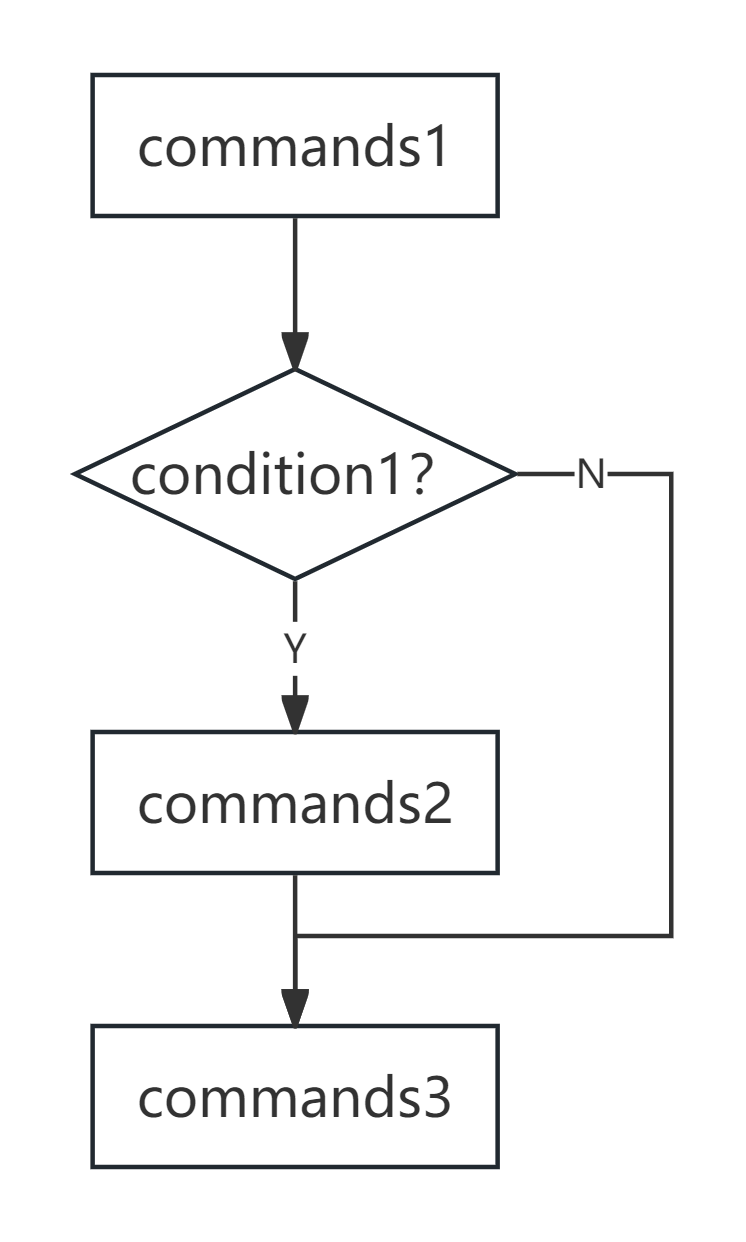
\includegraphics[width=1\linewidth]{Linux基础/Shell脚本基础/判断语句/fig/if语句.png}
    \caption{if语句流程图}
    \label{fig:判断语句-if语句流程图}
\end{figure}

这一段代码当执行完\code{commands1}之后,进行condition判断(条件是否成立),如果(if)成立,然后(then)执行\code{commands2}语句,\emph{否则不执行任何语句},最后执行\code{commands3}。

\begin{attention}
    无论条件是否满足,\code{commands3}都会执行(它是if语句之外的内容,类似于\code{commands1})。在这里的\code{commands1,commands2,commands3}都代表语句(们),每一部分可以是一条或多条语句。\code{condition}是\emph{判断条件},在后面的部分我们将详细介绍如何描述这一部分,简单来说,它描述的内容就是“是否……?”。

    需要特别注意\code{condition}前后与中括号之间的空格,这个空格不能省略!千万不要写成\code{[condition]}这种形式。
\end{attention}

\begin{extend}
    与C语言使用大括号,Python语言使用缩进不同,Shell脚本采用类似于Basic语言和MATLAB那样使用语句表示一整个语句块的方式。一个判断语句一定是以\code{if}开始,以\keyword{fi}结束。这个\code{fi}不代表“finish”或者“final if”等类似含义,而是\code{if}的倒序(在后面其他内容的学习中,会逐渐印证这一点)。

    换言之,在上述代码中,使用缩进与否并不会影响脚本执行效果,但为了增强可读性,我们仍然建议\emph{使用缩进表示每一级之间的层级关系}。事实上,如果你使用\code{vi}创建\code{*.sh}文件时,在输入\code{if}后默认会进行缩进,这也是大多数现代程序语言文本编辑器应当具有的功能。
\end{extend}

\subsection{关系运算符}\label{subsec:判断语句-关系运算符}

任何一个分支判断语句,都应当首先给定一个关系运算,并根据这个结果来判断应该执行哪些命令。在Shell脚本中,我们大致可以将关系运算符分成三类:

\subsubsection{整数比较}

类似于数学上的大于、小于和等于,在Linux当中也有对数值的比较,包括等于(\code{-eq}, \code{==})、不等于(\code{-ne}, \code{!=})、大于(\code{-gt}, \code{>})、小于(\code{-lt}, \code{<})、大于等于(\code{-ge})和小于等于(\code{-le})六种。

\begin{attention}
    在Shell脚本中,许多运算符都是通过上面这种“选项”的形式给出。与一般输入命令类似,选项前后也需要有空格进行分割。

    除了选项格式外,前四种(等于、不等于、大于和小于)我们也给出了类似于C和Python等其他编程语言所使用的运算符格式。这些在Shell脚本中同样可用。但是,对于大于等于和小于等于,没有\code{>=}和\code{<=}。如果你使用了这两个符号,大概率会报错。关于这一问题,目前还没有找到相关的解决方法,如果你有了对应解决方法(当然,不是后面要讲的内容),请联系我。
\end{attention}

\begin{extend}
    这些选项实际上是英文单词的缩写,例如,\code{eq}=equal; \code{ne}=not equal; \code{gt}=greater than; \code{lt}=less than; \code{ge}=Greater or Equal; \code{le}=Less or equal

    在后面你还会见到其他类似的语句,了解它们的实际含义可以帮助你记忆这些选项。
\end{extend}

下面的程序可以用来判断两个数字是否相等(使用前面的\code{if}语句)

\begin{lstlisting}[language=bash,caption=if\_equal,numbers=left]
#!/bin/bash
# 判断两个数字是否相等
a=10
b=10
# if语句判断是否相等
if [ $a -eq $b ]; then
    echo "$a is equal to $b"
fi
# 判断结束后输出
echo "Bye!"
\end{lstlisting}

你可以试着修改变量的值,查看输出结果是否有不同。在上述代码中,当变量相等时,判断结果为“1”,从而执行里面的语句;如果不相等,则判断结果为“0”,跳过里面的语句。无论结果如何,你都会看见第10行所输出的“Bye!”(它在\code{if}语句外面)。

\begin{extend}
    在这里我们提到了“1”和“0”,它们实际上叫做“\emph{布尔值}”或者“\emph{逻辑值}”,也是关系运算(与后面要提到的逻辑运算)的返回结果,其值只包含两种:“真”(也可以用“True”、“1”等代替)和“假”(也可以用“False”、“0”等代替)。
\end{extend}

\begin{attention}
    在中括号里面表示条件判断时,请务必记得中括号内前后要加空格,同时\code{-eq}前后也要加空格。

    在完成\code{if}语句后,不要忘记后面的\code{fi}。
\end{attention}

你也可以试着修改判断条件,例如改成\code{-gt},并修改变量的值,查看结果。

\subsubsection{*浮点数比较}

\begin{extend}
    由于前面所介绍的浮点数在脚本中的局限性,这一部分内容关于浮点数的比较并非必须了解。但如果你确实有此方面需求,在确定不能使用其他如C和Python等编程语言实现的前提下,可以参考这一部分所介绍的方法。

    相比于前面的整数比较,浮点数比较\emph{不能使用}前面的“选项”格式。例如,你写出\code{if [ 3.5 -ne 2.5 ]}是错误的。但是,前面所使用的运算符形式如\code{==, !=}等还是可用的。基于此,对于判断等于和不等于(包括大于和小于),最简单的方法就是使用如\code{if [ 3.5 != 2.5 ]}的格式。

    但是,对于大于等于和小于等于这两种情况,整数部分尚且还有选项可用,浮点数则完全没有对应的简单方法。参考前面\ref{subsec:变量-变量简单运算}一节所介绍的\code{bc}命令,我们可以退而求其次,借助于逻辑运算符的输出结果1和0,来进行判断。例如,我们希望判断3.5是否大于等于2.5,则可以使用\code{if [ \$(echo "3.5 >= 2.5" | bc) -eq 1 ]}这种方式,其中小括号部分借助管道运算符和\code{bc}命令计算\code{3.5 >= 2.5}的结果,根据前面所介绍的逻辑值,输出结果应当是0或1(在这里为1)。然后利用整数的判断方法,判断它与0或1的关系,从而实现浮点数对大于等于和小于等于的判断。
\end{extend}

\subsubsection{字符串判断}

与数值判断类似,字符串也可以进行相应的判断,一般常见的包括判断两个字符串是否相等(\code{==}),是否不相等(\code{!=}),以及判断一个字符串是否为空字符串(\code{-z}和\code{-n})

\begin{attention}
    在判断是否为空字符串时,可以使用\code{-z}和\code{-n},二者在本质上判断的内容是一样的,但返回结果\emph{相反},前者当内容为空时返回“真”,后者当内容不为空时返回“真”。借助于后面的“求非”运算,这二者只需要有一个即可,但为了简洁易读,还是建议在对应的时候使用正确的关系运算符。

    此外,与前面数值判断不同,判断字符串是否为空是“一元运算符”,即\emph{只需要一个变量}。后面的代码则给出了这种一元运算符的一般格式。
\end{attention}

下面的代码实现了判断一个字符串是否为空字符串:

\begin{lstlisting}[language=bash,caption=string\_empty,numbers=left]
#!/bin/bash
# 判断字符串是否为空
read -p "Please input a string:" string
# -n当字符串不为空时为真
if [ -n "$string" ]; then
    echo "Right! I got something ..."
    echo "You input: $string"
fi
echo "Bye!"
\end{lstlisting}

上述代码第5行通过\code{-n}判断输入字符串是否不为空,如果有内容(结果为真),则执行\code{if}语句里面的内容。

\begin{attention}
    在对字符串进行判断时(包括使用二元关系运算符),请务必将字符串变量前后加上双引号。如果不加双引号可能会造成奇怪的错误。
\end{attention}

\subsubsection{文件判断}

Shell脚本也提供了大量的运算符选项,用来判断文件的相关信息。例如,使用\code{-e}判断文件\emph{是否存在},使用\code{-f}(\code{-d})判断是否为普通文件(目录),使用\code{-r, -w, -x}依次判断文件是否可读、可写、可执行。

与前面字符串的代码类似,这里的所有运算符都是一元运算符(即采用\code{<选项> 变量}的格式。例如,下面的代码简单实现了判断文件\code{INCAR}是否存在的功能:

\begin{lstlisting}[language=bash,caption=file\_exist,numbers=left]
#!/bin/bash
# 判断文件INCAR是否存在
if [ -e "INCAR" ]; then
    echo "This file exists."
fi
echo "Bye!"
\end{lstlisting}

其中,\code{-e}后面的\code{"INCAR"}是指当前运行目录下的INCAR文件,你也可以使用绝对路径来描述文件。

\subsection{带有\keyword{else}的判断语句}\label{subsec:判断语句-带有else的判断语句}

下面,我们将进一步介绍\code{if}语句,在之前我们仅仅用来判断某一个条件是否满足,且当满足时执行某一(些)语句。但有时,我们可能有更复杂的需求。例如,判断某一个文件是否存在,如果存在则对文件进行处理,如果不存在则输出文件不存在,并提示用户重新输入。我们姑且忽略到继续输入这一动作(需要用到后面的循环),当条件不满足时如何执行另外的语句?类似于其他编程语言,在Shell当中也可以使用\code{if-else}语句。其基本格式如下:

\begin{lstlisting}[language=bash]
commands1
if [ condition ]; then
    commands2
else
    commands3
fi
commands4
\end{lstlisting}

\begin{figure}
    \centering
    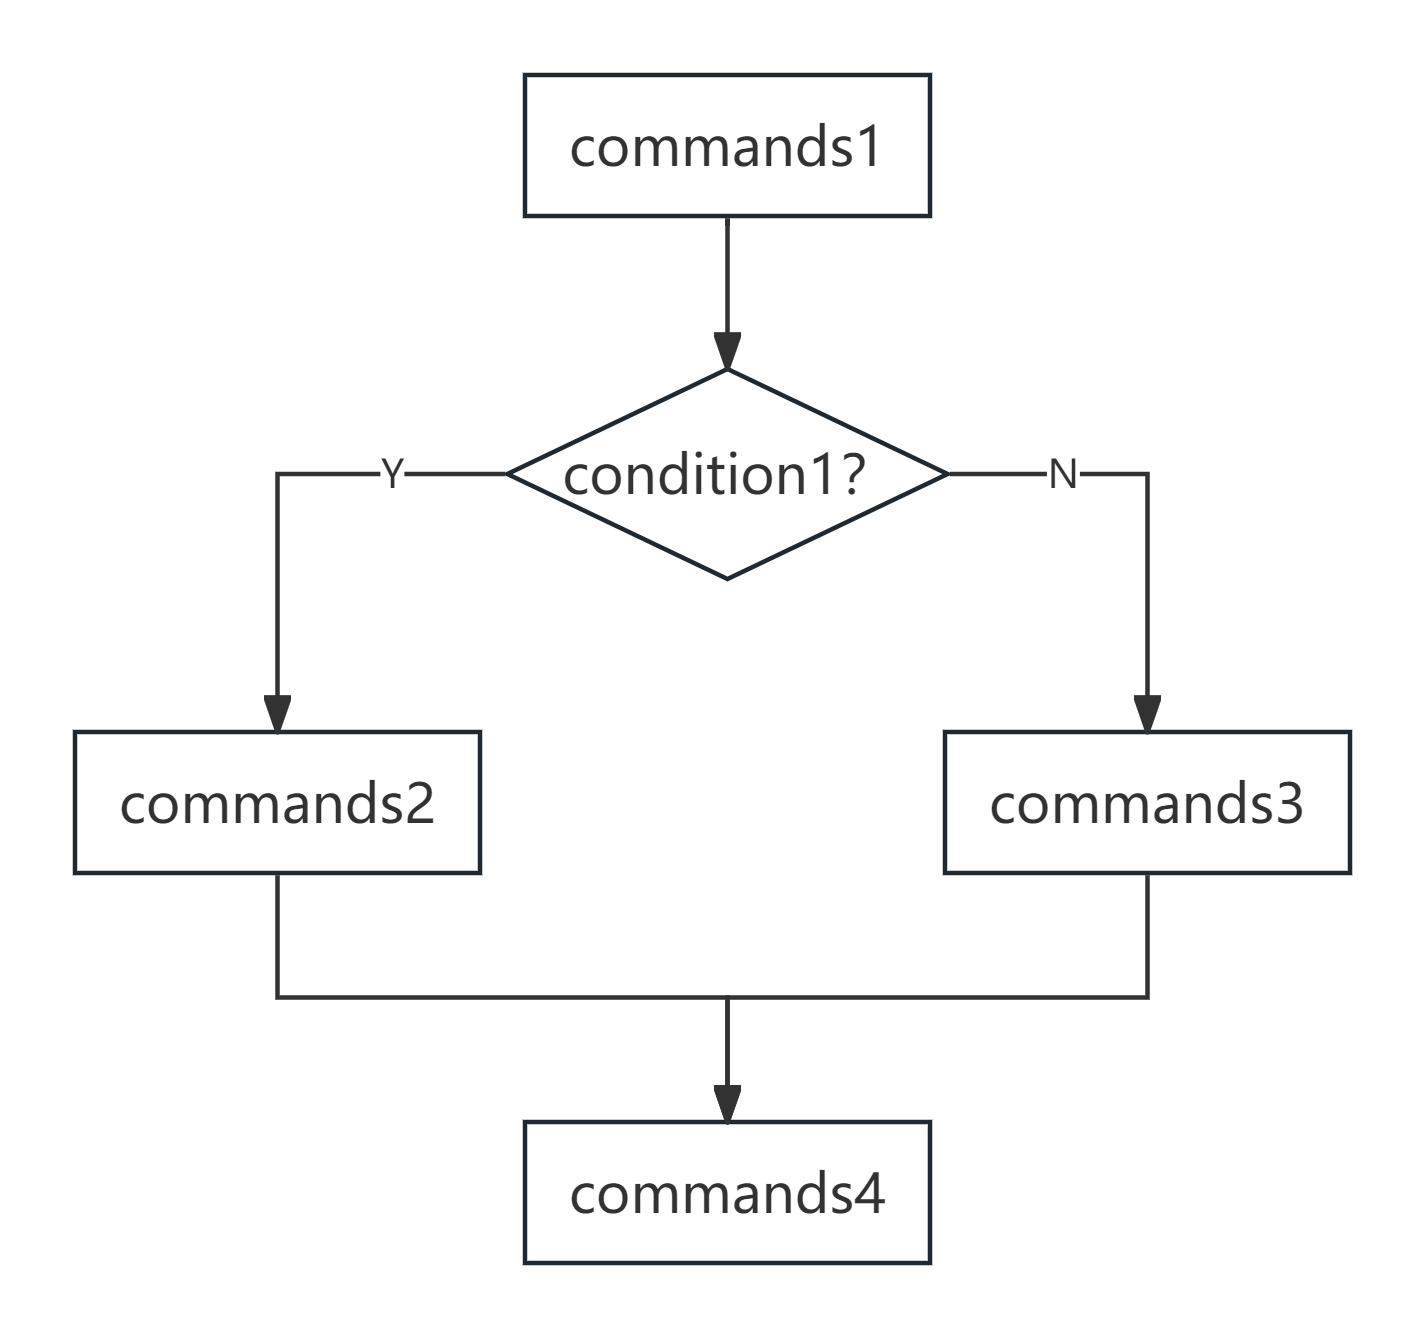
\includegraphics[width=1\linewidth]{Linux基础/Shell脚本基础/判断语句/fig/if-else语句.png}
    \caption{if-else语句}
    \label{fig:判断语句-if-else语句}
\end{figure}

首先程序会执行\code{commands1},然后进行判断,如果(if)条件成立,则(then)执行\code{commands2},否则(else)执行\code{commands3}。 无论结果如何,最后执行\code{commands4}。

下面的代码则是利用上面的语法结构,对前面的判断文件是否存在的脚本(file\_exist)进行了修改:

\begin{lstlisting}[language=bash,caption=file\_exist(2),numbers=left]
#!/bin/bash
# 判断文件INCAR是否存在
if [ -e "INCAR" ]; then
    echo "This file exists."
else
    echo "This file NOT exists."
fi
echo "Bye!"
\end{lstlisting}

除此之外,与Python语言类似,Shell脚本也有\code{if-elif-else}语句,用来对多条件进行判断,语法如下:

\begin{lstlisting}[language=bash]
commands1
if [ condition1 ]; then
    commands2
elif [ condition2 ]; then
    commands3
elif [ condition3 ]; then
    commands4
……
else
    commands5
fi
commands6
\end{lstlisting}

\begin{figure}
    \centering
    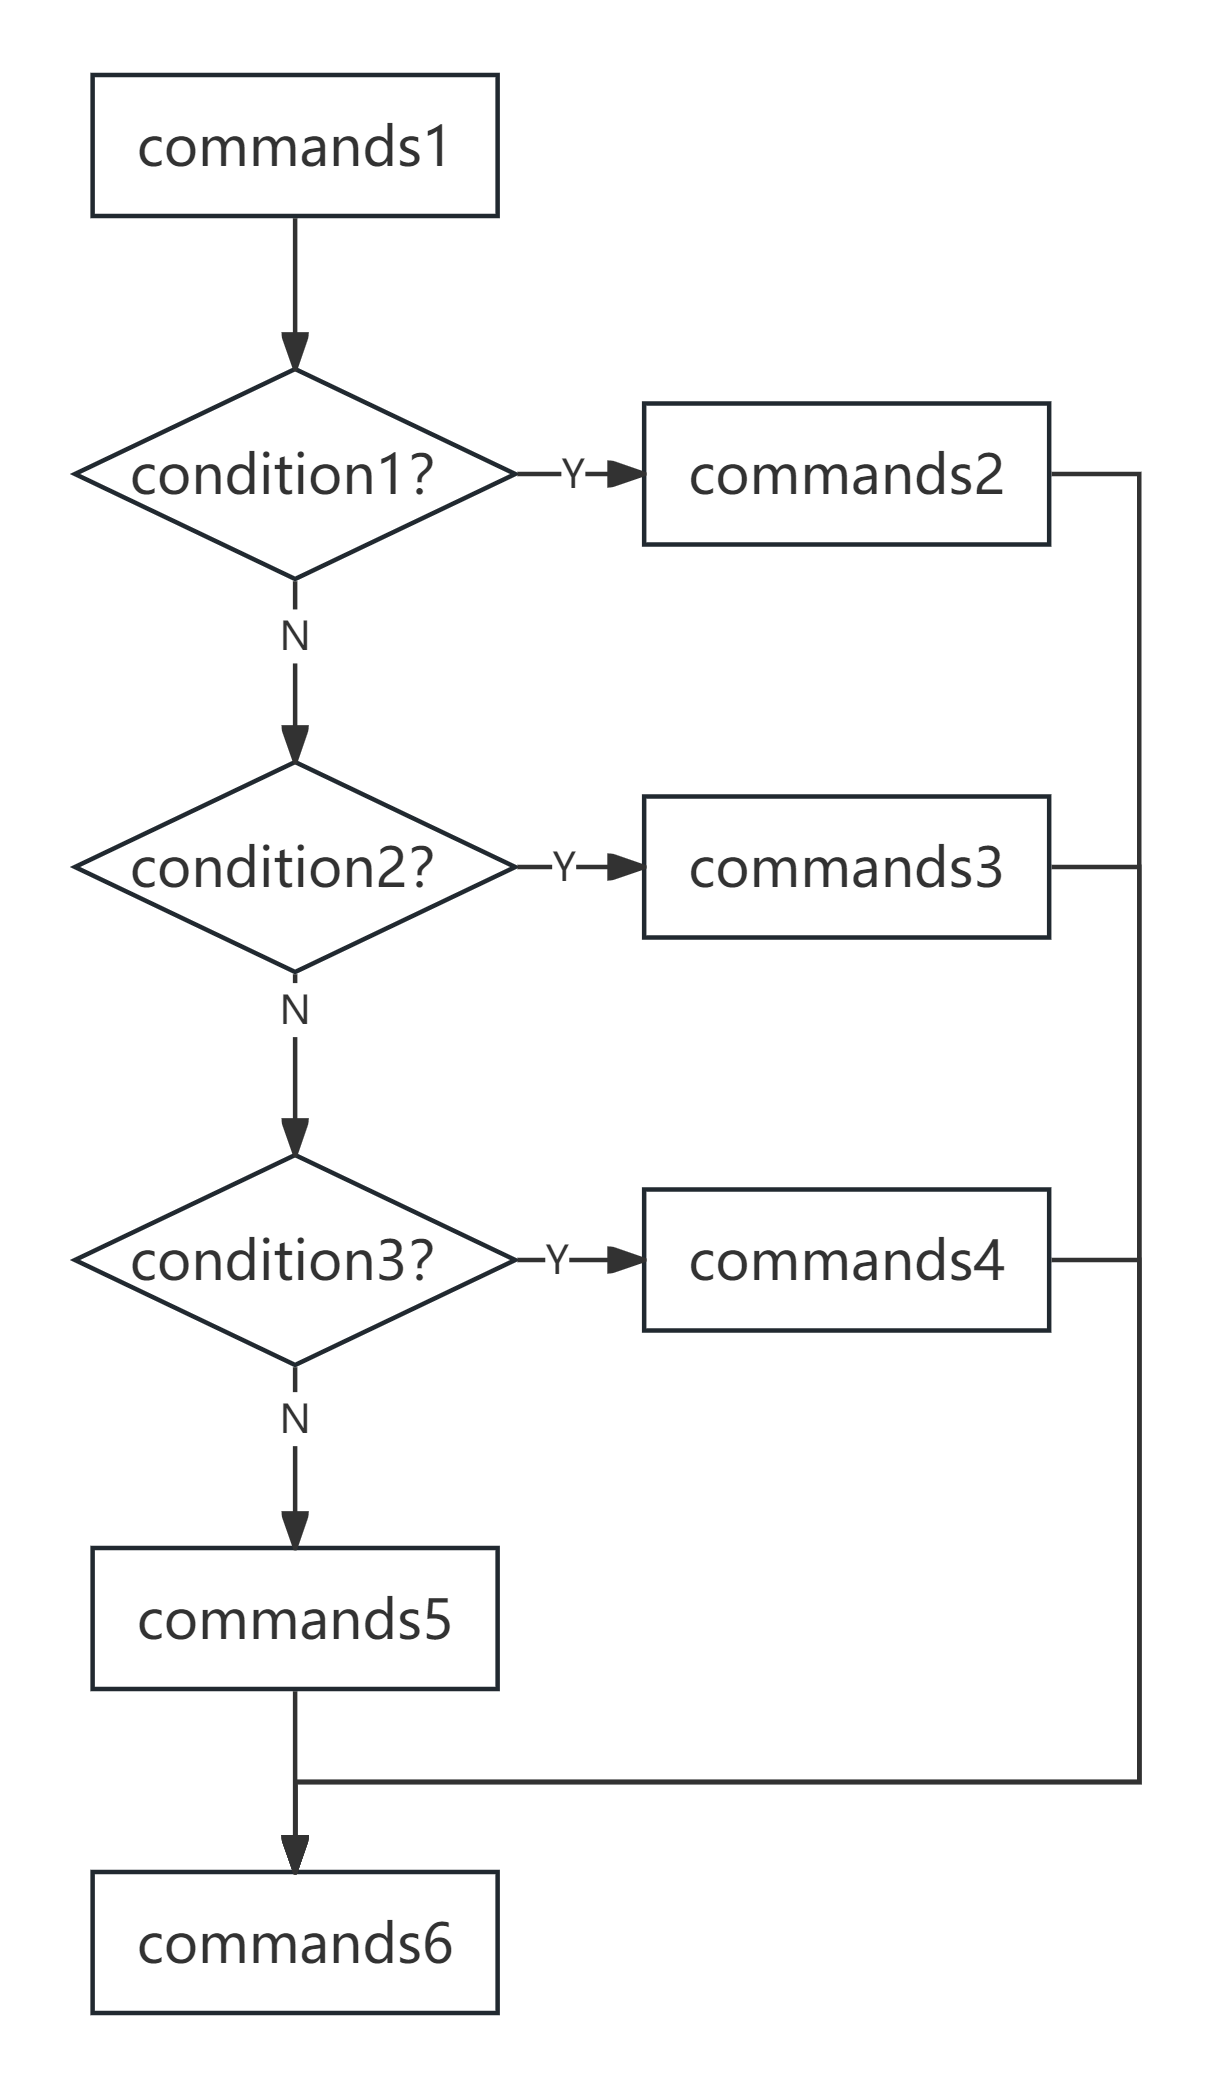
\includegraphics[width=1\linewidth]{Linux基础/Shell脚本基础/判断语句/fig/if-elif-else语句.png}
    \caption{if-elif-else语句}
    \label{fig:if-elif-else语句}
\end{figure}

程序首先判断\code{condition1}是否满足,如果(if)满足,则(then)执行\code{commands2}并结束判断语句,反之如果(else if, elif)满足\code{condition2},则(then)执行\code{commands3}并结束判断语句;反之如果……;否则都不满足(else),执行\code{commands5}。在结束判断语句后,执行\code{commands6}。

下面的程序可以用来判断两个整数之间的关系:

\begin{lstlisting}[language=bash,caption=compare\_number,numbers=left]
#!/bin/bash
# 判断两个整数之间的关系
# 输入两个整数
read -p "Please input an integer(a): " a
read -p "Please input an integer(b): " b
# 判断两个整数之间的关系
if [ $a -eq $b ]; then
    echo "$a = $b"
elif [ $a -gt $b ]; then
    echo "$a > $b"
else
    echo "$a < $b"
fi
echo "Bye!"
\end{lstlisting}

\subsection{嵌套\code{if}语句}\label{subsec:判断语句-嵌套if语句}

与其他编程语言类似,脚本也可以使用嵌套的\code{if}语句,甚至可以更复杂的\code{if-elif-else}嵌套,基于此可以实现复杂的功能。在这里我们不举例子,但有一个需要特别注意的地方:

\begin{attention}
    任何一个\code{if}语句,其后面都需要配合一个\code{fi}作为语句结束。尤其是对于嵌套时的\code{if-else}匹配问题,\code{else}总是与最近的未完成的\code{if}语句匹配(与缩进无关)。例如,下面的代码就违反了第一个原则(\code{if}必须配合有一个\code{fi});同时,看似\code{else}是属于\code{condition1}所对应的判断,但事实上是属于里面的\code{if}。

    \begin{lstlisting}
if [ condition1 ]; then
    commands1
    if [ condition2 ]; then
        commands2
else
    commands3
fi
    \end{lstlisting}

    这段代码是无法正常运行的。所缺少的\code{fi}可以加在\code{commands2}后面,也可以加在\code{commands3}后面,二者所实现的效果是不一样的。你可以尝试一下不同位置所对应的程序运行结果。

\end{attention}

\subsection{逻辑运算}\label{subsec:判断语句-逻辑运算}

在这一节的最后,让我们再来讨论一下逻辑运算。逻辑运算一共分为三种:与(\code{-a})、或(\code{-o})和非(\code{-n})。其中与运算和或运算都是二元运算符,而非运算是一元运算符。

对于与运算而言,\emph{只有当两个值都为真时结果为真}。而对于或运算,\emph{只要有一个为真,结果为真}\footnote{或者还有一种表述是,只有当两个值都为假时,结果为假。}。对于非运算,是一元运算符,其运算结果就是\emph{真变假,假变真}。

下面一个例子实现了判断三个数字是否从小大大排序:

\begin{lstlisting}[language=bash,caption=sort,numbers=left]
#!/bin/bash
# 判断三个数字是否从小到大排序
a=5
b=8
c=10
# 使用与运算符连接
if [ $a -le $b -a $b -le $c ]; then
	echo "$a, $b, $c"
fi
\end{lstlisting}

\begin{extend}
    在这里我们使用多个运算符进行连接,与其他编程语言类似,这里也具有“优先级”的问题。可以简单的理解:关系运算符的优先级高于逻辑运算符的优先级(这在大多数编程语言中都是如此)。虽然上面的写法比较简单,但对于条件复杂的时候可能不具有较好的可读性。因此,可以使用类似于C语言的运算符(\code{\&\&}表示“与”,\code{||}表示“或”),而中间每一个条件使用中括号分割,写作\code{if [ \$a -le \$b ] \&\& [ \$b -le \$c ]}
\end{extend}


\subsection{错误处理}\label{subsec:判断语句-错误处理}
% 请在本节列出可能遇见的错误与解决方法

这一部分有可能出现的错误太多了,以至于难以在这里全部列出。这里仅列举一些常见的错误,且这些错误的解决方法仅是一部分可能的原因。当你出现错误时,请首先查看对应的格式是否正确,并且可以尝试联系我们。

\subsubsection{-bash: <文件名>: line <行号>: syntax error: unexpected end of file}

这是因为在使用\code{if}后没有对应的\code{fi}作为结束。通常出现在嵌套语句中或者一个\code{if}语句太长,到最后忘记了匹配。对此,我们建议,在开始就按照\code{if-fi}对应关系输入。

\subsubsection{bash: [<变量>: command not found...}

这可能是由于你在输入关系表达式时忘记了中括号里前后要加空格。

\subsubsection{-bash: [: missing `]'}
与前面的错误类似,这个通常指右中括号前面没有空格。
% 请在下方的大括号相应位置填写正确的节标题和标签,以及作者姓名
\section{\keyword{case}分支语句}\label{sec:case分支语句}
\sectionAuthor{Jiaqi Z.}

% 请在下方的item内填写本节知识点
\begin{Abstract}
    \item 如何使用\code{case}语句实现分支判断
\end{Abstract}

在前面的\code{if}语句中,已经了解了如何进行判断。理论上了解了\code{if}语句后可以解决所有分支情况,但是有一些情况可能比较特殊。例如,我们希望实现一个菜单界面,此时可能需要用户输入一些指令表示对应的功能。可以想见,如果使用\code{if}语句,将会有许多的判断条件,甚至随着条件的增多,也会影响程序运行效率\footnote{这是因为在进行判断时,脚本需要对所有条件进行遍历。}。

因此,我们希望可以寻找一种方法,直接对变量进行判断,并根据它的值选择合适的语句执行。可以猜到,这就是本节\code{case}语句所要解决的问题。

\subsection{\code{case}语句基本结构}\label{subsec:case分支语句-case语句基本结构}

类似于\code{if}判断语句,\code{case}判断语句的基本结构为:

\begin{lstlisting}[language=bash]
case <变量> in
pattern1)
    statements1
    ;;
pattern2)
    statements2
    ;;
......
*)
    statements3
    ;;
esac
\end{lstlisting}

程序会根据变量所在(in)的模式(可以是一个单独的值,或者正则表达式),选择合适的语句进行执行。例如,如果变量满足\code{pattern1},则会执行\code{statements1}语句;如果满足\code{pattern2},则会执行\code{statements2}语句;以此类推,如果所有的都不满足,则执行\code{*}所对应的\code{statements3}语句。

\begin{attention}
    有几个细节需要特别关注:所有匹配模式都是以小括号作为结束分割(没有左括号);当每一个分支里面的语句结束时,需要有\code{;;}作为结束的标志;在\code{case}语句结束时,需要有\code{esac}作为结束标志。
\end{attention}

\begin{extend}
    正如在\ref{sec:判断语句}中所讲的那样,\code{esac}也是\code{case}的倒序。另外,模式当中的\code{*}实际上可以想见,表示的就是通配符里面的可以表示任意多个字符的\code{*}符号。
\end{extend}

\subsection{\code{case}语句应用}\label{subsec:case分支语句-case分支语句应用}

下面让我们来看几个常见的应用例子。

\subsubsection{单一字符匹配}

在\code{case}语句中,最简单的就是对单独一个字符进行匹配。下面这个例子则实现了一个对菜单的模拟,用户通过输入1或者2来实现对应不同的功能。

\begin{lstlisting}[language=bash,caption=simple\_menu,numbers=left]
#!/bin/bash
# 模拟菜单选项
echo "--------------------"
echo "1) option 1"
echo "2) option 2"
echo "--------------------"
read -p "Please input a number: " number
case $number in
1)
    echo "You input 1"
    echo "I will do something for option 1..."
    ;;
2)
    echo "You input 2"
    echo "I will do something for option 2..."
    ;;
*)
    echo "You did NOT input 1 or 2"
    ;;
esac
echo "Bye!"
\end{lstlisting}

运行上面的代码,可以看见:当用户输入1时,程序可以直接跳转到\code{1)}所对应的语句;对应的,当用户输入2时,可以跳转到\code{2)}所对应的语句;如果输入其他内容(例如输入3),则会跳转到最后提示输入错误。

\begin{attention}
    与\code{if}语句类似,\code{case}语句的前后,即开始的提示和后面的“Bye!”无论哪种情况都会输出,因为它们不属于\code{case}语句内。
\end{attention}

\subsubsection{字符串匹配}

字符串匹配与单一字符匹配完全一样(你可以将单个字符理解成一种特殊的字符串)。但是,在这里我们也有一点新东西要讲。如果我们希望多个选项匹配同一个分支,可以\emph{使用\code{|}符号表示“或”进行分隔}。例如,下面的程序则是根据用户输入的字符串选择特定的分支(有时多个输入对应同一个分支):

\begin{lstlisting}[language=bash,caption=favourite\_band,numbers=left]
#!/bin/bash
# 字符串匹配
read -p "Please input you favourite band: " band
case $band in
"PPP"|"ppp"|"Poppin'Party")
    echo "Thanks! I have known that you like Poppin'Party!"
    ;;
"Roselia"|"R")
    echo "Thanks! I have known that you like Roselia!"
    ;;
"RAS"|"RAISE A SUILEN"|"Raise a suilen")
    echo "Thanks! I have known that you like RAISE A SUILEN!"
    ;;
"MyGO!!!!!"|"mygo"|"mygo!!!!!")
    echo "Thanks! I have known that you like MyGO!!!!!"
    ;;
*)
    echo "Sorry...I don't know this band."
    echo "But now I have known it -- $band"
    echo "Thank you!"
    ;;
esac
echo "Bye!"
\end{lstlisting}

与前面的代码分析完全类似,但特别的是,这里面分支的判断使用\code{|}表示“或”,例如,“PPP”、“ppp”和“Poppin'Party”对应的都是同一个分支;类似地,“R”和“Roselia”也是对应同一个分支,当用户输入“R”或者输入“Roselia”时,得到的结果是一样的。

\subsubsection{正则表达式匹配}

正如一开始所说的那样,在匹配时可以使用\emph{正则表达式}。例如,下面的代码试图读取用户输入的参数为字母还是数字\footnote{为了复习之前的变量种类,我们在这里尝试使用参数给定变量而不是使用\code{read}命令。}:

\begin{lstlisting}[language=bash,caption=number\_or\_letter,numbers=left]
#!/bin/bash
# 读取调用时的选项
export LC_ALL=C
case $1 in
[a-z])
    echo "You input a lowercase"
    ;;
[A-Z])
    echo "You input an uppercase"
    ;;
[1-9])
    echo "You input a number"
    ;;
*)
    echo "You input other things"
    ;;
esac
echo "Bye!"
\end{lstlisting}

\begin{extend}
    也许你足够灵敏,注意到了第3行的\code{export LC\_ALL=C},这句命令表示将程序运行语言环境设置为默认值(可以通过\code{locale}查看环境语言设置),其中\code{C}表示系统默认值。
    
    在这里我们需要添加这一行命令以确保程序运行正确,但这行命令并不影响我们对\code{case}的理解。

    同时,当你运行这一行代码之后,可能程序中的中文注释发生乱码,这并不影响程序运行结果,你可以重新启动系统以恢复开始的状态。
\end{extend}

在调用时,当用户传递给一个小写字母时,则会匹配到\code{[a-z]},相对地,若给定一个大写字母作为参数,则会匹配到\code{[A-Z]}。但是,我们这里只能对用户输入的一个参数进行判断,如果用户输入多个字符的参数(例如\code{abc}),程序则会认为输入了其他内容。如何修改程序呢?请自己思考并尝试写一段代码\footnote{请真的这样做,这会极大提高你的编程思维。},同时自己测试它。(为简单起见,我们只需要匹配第一个字符即可)

同时,正则表达式也可以使用\code{|}作为分隔以进行多个情况的判断,例如,我们希望将上面的代码修改为无论大小写字母都判断为字母,则可以写成下面的样子:

\begin{lstlisting}[language=bash,caption=number\_or\_letter2,numbers=left]
#!/bin/bash
# 读取调用时的选项
export LC_ALL=C
case $1 in
[a-z]|[A-Z])
    echo "You input a letter"
    ;;
[1-9])
    echo "You input a number"
    ;;
*)
    echo "You input other things"
    ;;
esac
echo "Bye!"
\end{lstlisting}


\subsection{错误处理}\label{subsec:分支语句-错误处理}
% 请在本节列出可能遇见的错误与解决方法

\subsubsection{-bash: <文件名>: line <行号>: syntax error near unexpected token `)'}

这可能是因为你在结束分支时少了\code{;;}表示当前分支内结束。如果你了解C语言,你可能会很自然将这这个符号作为C语言中\code{switch-case}的\code{break}语句。但显然,C语言的\code{break}更加灵活(它可以没有从而越过其他分支),但Shell脚本不能没有\code{;;}结束。

\subsubsection{-bash: <文件名>: line <行号>: syntax error near unexpected token `<字符串>'}

这可能是由于你在使用\code{case}语句后忘记结束\code{esac}而后面还有其他语句从而报错。如果后面没有语句,则可能会出现下面的错误:

\subsubsection{-bash: <文件名>: line <行号>: syntax error: unexpected end of file}

这也表明你可能没有使用\code{esac}作为\code{case}语句的结束。
% 请在下方的大括号相应位置填写正确的节标题和标签,以及作者姓名
\section{循环}\label{sec:循环}
\sectionAuthor{Jiaqi Z.}

% 请在下方的item内填写本节知识点
\begin{Abstract}
    \item 如何使用\code{for}循环
    \item 如何使用\code{while}循环
    \item 如何使用\code{until}循环
    \item \code{while}循环和\code{until}循环的区别
\end{Abstract}

在前面介绍高级Linux命令时,我们曾说过脚本处理的任务大多是\emph{批量处理}任务,而批量处理的一个基本方法就是使用循环语句(毕竟没有人会想写上上百行相同的代码)。在\ref{sec:简单for循环}一节中,我们介绍过\code{for}循环的使用,当时是在命令行中编写的。本节我们将首先复习一下\code{for}循环的基本使用方法,以及它在脚本程序中的格式(和命令行类似),然后再介绍两种不同的循环语句——\code{while}循环和\code{until}循环——它们虽然在一定程度上是等价的,但在不同的情况下,选择合适的循环语句会让程序更加简洁易读。

\subsection{\code{for}循环}\label{subsec:循环-for循环}

下面的代码完整演示了常见的三种\code{for}循环格式:

\begin{lstlisting}[language=bash,numbers=left,caption={for\_example}]
#!/bin/bash
# 使用for循环输出
# 简单列表
for i in 1 2
do
    echo $i
done
echo ""
# 生成列表
for i in $(seq 1 2 10)
do
    echo $i
done
echo ""
# 使用C语言格式
for ((i=0;i<10;i++))
do
    echo $i
done
\end{lstlisting}

其中第8行、第14行使用\code{echo ""}输出一个空行用来区分不同的输出结果。

\subsubsection{简单列表}

使用基本列表的格式调用\code{for}循环的基本格式为:

\begin{lstlisting}[language=bash]
for <变量名> in <列表>
do
    循环体
done
\end{lstlisting}

\begin{extend}
    在循环语句内部的语句,我们常常称其为\emph{循环体}(实际上和前面所说的\code{commands},程序块,语句块等一样)
\end{extend}

在这里的\code{<列表>}可以如同上面的代码一样直接以空格分隔表示,也可以与\ref{sec:简单for循环}一节所说的那样使用大括号将其括起来,并用逗号分割。

\begin{attention}
    一个常见的错误是将两者混淆,即\emph{使用大括号表示列表的同时,其内部元素用空格分隔}。可以验证的是,这并不会如你所愿得到正确的信息。事实上,空格的“优先级”会高于大括号的“优先级”(这里加引号表示这不是传统意义上运算符的优先级),当括号和空格同时存在时,程序会将列表解析为\emph{以空格分隔的列表},从而在输出的前后(第一个元素和最后一个元素)带有大括号。
\end{attention}

与前面的介绍类似,在循环体内使用变量需要加\code{\$}符号。

\subsubsection{生成列表}

与\ref{sec:简单for循环}里所介绍的方法类似,可以使用\code{seq}命令生成序列。与前面所介绍的方法不同的是,前面所使用的是\code{`}符号括起来的命令,而在脚本中,由于将\code{seq}看作是一个命令,因此与前面\ref{subsec:输入-读取命令作为输入}一节所介绍的输入方式类似,使用\code{\$()}的方式得到\code{seq}命令的结果,并将其作为一个变量传递给\code{for}循环。

当然,也可以使用前面所说的\code{..}的方式生成序列。但需要复习的是:对于\code{seq}语句而言,三个参数分别是\emph{开始、步长、结束};而对\code{..}方式而言,三个参数分别是\emph{开始、结束、步长}。因此,上面代码的\code{seq 1 2 10}也可以写作\code{\{1..10..2\}}

\subsubsection{运算格式生成}

如果你熟悉C语言的话,这一种格式会显得很“亲切”。因为它的基本结构与C语言几乎完全类似,类似地写法,如果让我们用C语言实现上面代码的第3部分,则可以写作这样:

\begin{lstlisting}[language=C,numbers=left]
#include <stdio.h>
void main()
{
    for (int i=0;i<10;i++)
        printf("%d\n",i);
}
\end{lstlisting}

可以看到,相比于C语言,脚本只是一个括号和两个括号的区别\footnote{由于C语言是强类型语言,因此在for循环条件中定义了变量类型\code{int},但这不是必需的,因为完全可以将变量定义放在循环外面作为单独的语句,此时C语言的括号内与脚本的括号内就完全相同了。在比较二者不同时,我们有意忽略了这一点,只是为了让大家关注到本质}。

\begin{attention}
    在脚本的\code{for}循环当中,括号前面没有\code{\$}符号,也千万不要“画蛇添足”加上这个符号。
\end{attention}



\subsection{\code{while}循环}\label{subsec:循环-while循环}

与C语言的\code{while}循环类似,在bash脚本中也存在根据条件判断循环与否的\code{while}循环。其基本格式如下:

\begin{lstlisting}[language=bash]
while [ condition ]
do
    循环体
done
\end{lstlisting}

其中,\code{condition}表示\emph{循环进行的条件},其格式与\ref{sec:判断语句}当中所介绍的条件表达式类似。例如,下面的代码实现了从0到9的输出

\begin{lstlisting}[language=bash,numbers=left,caption={while\_example}]
#!/bin/bash
# 使用while循环输出数字
i=0
while [ $i -lt 10 ]
do
    echo $i
    ((i++))
done
\end{lstlisting}

可以复习一下,条件\code{-lt}表示\emph{小于},因此,循环体进行的条件是\emph{变量\code{i}小于10}。当条件满足时,程序进行循环体(\code{do}和\code{done}中间的部分)。因此,程序会从0开始,逐渐输出并加1,直到条件不满足时(\code{i}为10)则停止循环。

\begin{attention}
    与\code{for}循环相比,\code{while}循环更有可能写出“死循环”语句。所谓“死循环”,指的是程序在循环体内一直循环,永无停止。在上面的代码中,如果少了那句\code{((i++))},则变量始终为0,条件始终满足,从而无法停止。

    具体的解决方法,可以见下一节所介绍的\code{break}和\code{continue}语句。
\end{attention}

此外,在上面程序的第7行,使用\code{((i++))}表示进行计算,这是比较简洁的C风格递增运算符,类似的还有递减运算符\code{--}。这种方式的使用需要以两个括号括起来。你也可以使用\ref{sec:变量}一节所介绍的方法,使用\code{i=\$(( \$i + 1 ))}的方式。这二者在这一功能上是等价的。

\subsection{\code{until}循环}\label{subsec:循环-until循环}

与\code{while}循环几乎完全类似,bash脚本中\code{until}循环的格式为:

\begin{lstlisting}[language=bash]
until [ condition ]
do
    循环体
done
\end{lstlisting}

与上面的\code{while}循环格式比较可以发现,除了关键字从\code{while}变成了\code{until}外,其他语句在格式上没有任何不同。但\code{until}循环的最大特点是:\emph{循环体执行的条件是\code{condition}为假},即你可以简单的将其理解为:循环体会一直执行,“直到”(until)条件为真。

\begin{attention}
    这一点稍微有点绕,但上面的两种表述是“等价”的。对\code{while}循环而言,当条件为真时执行循环体,而对\code{until}循环而言,当条件为真时退出循环(当条件为假时进入循环)
\end{attention}

\begin{extend}
    在C语言中,确实没有类似的循环与其对应,但我们可以从其他一些编程语言中找到这个例子,一个最简单的例子就是——Visual Basic语言(简称VB语言)。在VB语言中,也存在类似的\code{until}循环,其格式为:

    \begin{lstlisting}
Do 
    循环体
Loop Until 条件
    \end{lstlisting}

    如果你熟悉VB语言的话,bash脚本的\code{until}循环与VB语言的\code{until}循环最大的不同在于\emph{VB语言的条件是放在循环后面(类似于C语言的\code{do-while}循环)}

    当然,如果你不熟悉VB语言的话,也不必担心。这一部分仅仅是对那些熟悉VB语言的读者所准备的,以防他们混淆条件的位置。如果你本来不了解VB语言的话,这一部分完全可以跳过。
\end{extend}

可以简单想见的是,\code{while}循环和\code{until}循环之间的转换仅仅是“\emph{条件的取反}”,例如,上面关于\code{while}循环的例子,我们只需要将里面的条件\code{\$i -lt 10}改为\code{\$i -ge 10},同时将\code{while}改为\code{until}就可以实现相同的功能。这一部分代码我们不做演示,请自己尝试修改上面的代码并测试其输出结果是否与之前的结果一致。



% \subsection{错误处理}\label{subsec:节标题-错误处理}
% % 请在本节列出可能遇见的错误与解决方法

% \subsubsection{错误1}

% \subsubsection{错误2}

% \subsubsection{错误3}

    \part{VASP计算}

    \input{preface/vasp前言.tex}
\chapter{结构优化}\label{chap:结构优化}
\minitoc
% 请在下方的大括号相应位置填写正确的节标题和标签,以及作者姓名
\section{为什么要进行结构优化}\label{sec:为什么要进行结构优化}
\sectionAuthor{Jiaqi Z.}

% 请在下方的item内填写本节知识点
\begin{Abstract}
    \item 为什么要进行结构优化
    \item 结构优化的原理
\end{Abstract}

在计算科学领域,一个广为流传的话是“Garbage In, Garbage Out!”,即\emph{错误的输入会得到错误的结果}。因此,对材料计算而言,在进行任何材料计算之前,都需要保证输入的正确性,包括\emph{参数设置}的正确以及\emph{结构}的正确。其中,参数设置的正确性将取决于研究问题和研究经验,结构的正确则首先取决于\emph{结构优化}。本章我们将介绍关于结构优化的一些设置方法与技巧。

\begin{attention}
    在任何时候,开始一个新的体系进行计算,都需要进行本章所介绍的结构优化,哪怕这个材料是实验测得的或者数据库所给的。
\end{attention}

\subsection{为什么要进行结构优化}\label{subsec:为什么要进行结构优化-为什么要进行结构优化}

结构优化是指对整个输入体系的坐标进行调整,得到一个相对稳定的基态结构。例如,在计算材料的吸附性质时,我们需要通过结构优化得到一个“稳定”的吸附结构,从而测得吸附距离和其他稳定时的性质。如果需要确认材料的稳定性(例如计算声子谱),则显然需要首先进行结构优化以确保结构的“稳定”(甚至需要更高的精度)。

也许你会有一个疑问:\emph{如果结构已经实验测得,还需要结构优化吗}?答案是\emph{需要},这是因为计算软件本身是考虑了许多近似情况,有时实验测得的结构和计算所使用的稳定结构有“细微”的区别。例如,对于氧气分子而言,使用数据库(CCCBDB)内的数据,其键长为1.2075 Å. 当我们使用不同的近似(考虑不同类型的赝势)进行结构优化\footnote{这里我们仅作为示例给出结论,并不提供完整的输入文件。},得到的键长是不同的。使用O和O\_s的赝势,在设置截断能为600 eV的情况下,计算得到的键长分别为1.23828 Å和1.29688 Å.

上面的键长变化可以极好说明对于不同的参数设置以及近似条件,所得到的结构可能是不同的。因此,哪怕是实验测得的或者数据库所给的,在开始计算时也需要进行结构优化。

\subsection{结构优化原理}\label{subsec:为什么要进行结构优化-结构优化原理}

一个完整的结构优化计算,可以分为\emph{电子弛豫}和\emph{离子弛豫}两部分。首先,程序会计算许多步电子弛豫,以确定当前结构下稳定的波函数。基于密度泛函理论的基本原理,利用波函数可以得到体系的能量,判断能量是否达到极值点(大多数情况是判断原子平均受力);如果原子平均受力小于某一个设定的值,则认为结构已经“稳定”,否则会按照一定的算法对原子坐标进行移动,得到一个新的结构,再重复上述步骤,直到寻找到“稳定”结构。

\begin{attention}
    上面我们所说的“稳定”,指的是能量达到一个“极值点”。而利用基本的数学与物理相关知识可以知道,真正的稳定结构(基态)应当对应结构能量的“最小值”,而寻找到的“极值点”不一定是最小值。

    上述情况则会导致在有些情况下结构优化会得到一个“非最小值的极值点”,因此在实际计算时,可能还需要使用不同的初始结构进行结构优化,并通过能量比较确定最终的结构。一个典型的例子是计算吸附时需要考虑多个吸附位点,优化得到不同的结构,并通过能量比较确定最终的稳定吸附位点。
\end{attention}

% 请在下方的大括号相应位置填写正确的节标题和标签,以及作者姓名
\section{对坐标进行优化\code{ISIF=2}}\label{sec:对坐标进行优化ISIF=2}
\sectionAuthor{Jiaqi Z.}

% 请在下方的item内填写本节知识点
\begin{Abstract}
    \item 如何构建分子结构
    \item 如何对原子坐标进行结构优化
\end{Abstract}

本节,我们将实现\ref{subsec:为什么要进行结构优化-为什么要进行结构优化}中所介绍的氧气分子结构优化。首先,我们需要构建分子结构,并利用VASP进行结构优化,同时,我们将介绍如何查看关于结构优化的输出文件。需要特别注意的是,这一节的例子非常简单,但所介绍的内容(尤其是关于输出文件的理解)将有可能贯穿本章。

\subsection{构建氧气分子结构}\label{subsec:对坐标进行优化ISIF=2-构建氧气分子结构}

在VASP中,构建的所有结构都是需要基于\emph{晶胞}进行构建,即所有结构默认都是\emph{周期性结构}。有时,我们希望限制材料维数(例如二维材料、一维材料或分子、团簇),则需要在其他方向设置所谓的“真空层”以避免由于周期性所导致的材料之间的相互作用。

对于本节我们所考虑的氧气分子,由于是分子,因此在空间中可以是“孤立”存在的。在构建晶胞时在三个方向均设置较大的值以避免分子与分子之间的相互作用。在本例中,我们设置晶格常数为5 Å.

\begin{attention}
    VASP在POSCAR中没有\emph{晶系}的概念,构建的晶胞参数是基于“绝对空间坐标系”设置的。对于分子而言,晶系的设置不影响计算结果,我们可以设置为如三方晶系或更普通的三斜晶系等。但考虑到后续原子坐标设置方便,通常我们会将其设置为立方晶系。

    但如果需要考虑其他体系,例如材料吸附气体等情况,为后续能量具有可比较性,晶胞的设置需要参考其他材料(例如,根据衬底材料的晶胞设置气体分子所使用的晶胞)
\end{attention}

我们已经知道数据库内\ch{O2}分子的键长为1.2075 Å,因此,设置的\code{POSCAR}文件如下所示:

\begin{lstlisting}[caption=POSCAR]
O2
1.0
5.0 0.0 0.0
0.0 5.0 0.0
0.0 0.0 5.0
O
2
Cartesian
0 0 0
0 0 1.2075
\end{lstlisting}

这里为了设置方便,使用笛卡尔坐标设置原子坐标。在实际应用时,有时可能会借助其他软件如Materials Studio或者VESTA生成\code{POSCAR}文件,此时使用分数坐标(\code{Direct})也是可以的。

\begin{extend}
    如果你将上面的\code{POSCAR}文件放到VESTA文件进行预览的话,可能会发现有8个氧气分子(如图所示)。这并不是因为输入文件设置错了,而是因为VESTA在显示时考虑了周期性,8个氧气分子实际上是等价的。

    \begin{figure}
        \centering
        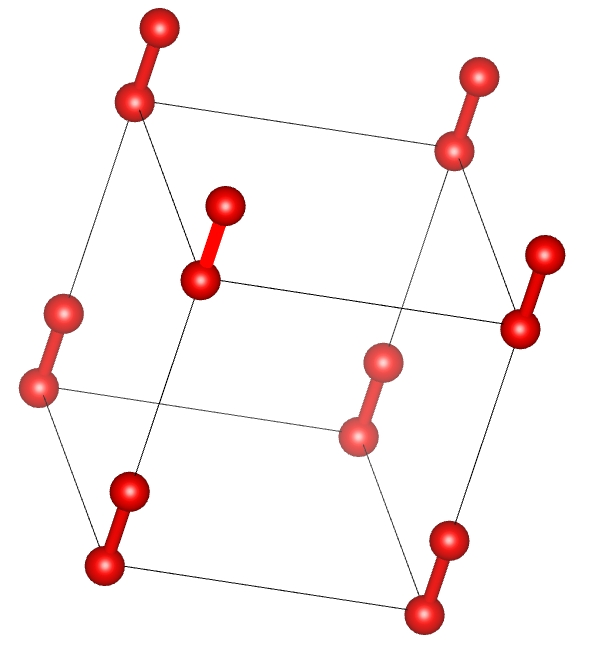
\includegraphics[width=0.5\linewidth]{VASP计算/结构优化/对坐标进行优化/fig/氧气分子.png}
        \caption{氧气分子}
        \label{fig:对坐标进行优化ISIF=2-氧气分子}
    \end{figure}
\end{extend}

\subsection{\code{INCAR}设置}\label{subsec:对坐标进行优化ISIF=2-INCAR设置}

下面是一个简单的\code{INCAR}文件

\begin{lstlisting}[caption=INCAR]
ENCUT  =  600
LWAVE  = .FALSE.
LCHARG = .FALSE.
PREC   = Accurate
NSW    =  300
ISMEAR =  0
SIGMA  =  0.05
IBRION =  2
ISIF   =  2
EDIFFG = -0.01
\end{lstlisting}

\begin{itemize}
    \item \code{ENCUT}:截断能(单位:eV),根据所使用的\code{POTCAR}文件所决定,需要大于所使用\code{POTCAR}当中所有元素\code{ENMAX}的最大值,且通常至少为1.3倍的\code{ENMAX}。在本例中我们设置为600 eV;
    \item \code{LWAVE}和\code{LCHARG}:是否输出\code{WAVECAR}和\code{CHGCAR}文件(分别为波函数和电荷密度)。由于结构优化时通常不关心这些文件,因此设置为\code{.FALSE.}节省硬盘空间;
    \item \code{PREC}:计算精度,在进行结构优化时,为确保结构合理,通常设置为\code{Accurate};
    \item \code{NSW}:离子弛豫的最大步数。如\ref{subsec:为什么要进行结构优化-结构优化原理}中所介绍的那样,结构优化需要进行多步离子弛豫直到收敛。若离子弛豫步数达到\code{NSW}则直接停止(哪怕没有收敛);
    \item \code{ISMEAR}:决定在布里渊区积分时,如何计算分布函数。当设置为0时表示使用Gaussian展宽,其展宽宽度由\code{SIGMA}参数决定(单位:eV);
    \item \code{ISIF}:设置为2表示仅优化原子坐标,不优化晶格;
    \item \code{EDIFFG}:当设置为正值时表示能量收敛标准,当设置为负值时表示原子之间的作用力收敛标准。
\end{itemize}

在本例中,我们设置\code{ISIF=2},这是由于我们所优化的结构为分子体系,并不希望优化外面的晶格参数。除此之外,\code{ISIF}还有其他参数(常见的可能设置为3,在下一节介绍)。同时,通过设置\code{EDIFFG}决定收敛精度,通常设置为\code{-0.01}就已经达到了一般研究所需要的精度,但对于更高精度需求(例如计算声子谱),则可能需要到\code{-1E-3}的精度。

在实际使用时,可以考虑使用VASPKIT,使用\code{vaspkit-101-LR}或者\code{vaspkit-101-SR},其中前者默认设置\code{ISIF=3},而后者设置\code{ISIF=2}

\subsection{其他输入文件}\label{subsec:对坐标进行优化ISIF=2-其他输入文件}

由于计算的是分子体系,不需要考虑周期性,因此在计算时\code{KPOINTS}的设置仅使用Gamma点即可。在生成时可以使用\code{vaspkit-102-2-0}生成Gamma点的\code{KPOINTS}。调用这个命令的同时也会生成默认的\code{POTCAR}文件。

\subsection{计算结果分析}\label{subsec:对坐标进行优化ISIF=2-计算结果分析}

对于结构优化,我们重点关注\code{OSZICAR}和\code{CONTCAR}文件。执行上面的任务,所得到的\code{OSZICAR}文件如下所示(仅供参考):

(为排版方便,对小数点进行了截断处理)

\begin{lstlisting}[caption=OSZICAR,basicstyle=\tiny]
        N       E                     dE             d eps       ncg     rms          rms(c)
DAV:   1     0.281908272337E+02    0.28191E+02   -0.56622E+03   192   0.105E+02
DAV:   2    -0.903395442264E+01   -0.37225E+02   -0.37218E+02   288   0.201E+01
DAV:   3    -0.907739062911E+01   -0.43436E-01   -0.43400E-01   192   0.111E+00
DAV:   4    -0.907742563069E+01   -0.35002E-04   -0.35001E-04   384   0.308E-02
DAV:   5    -0.907742563010E+01    0.58537E-09   -0.20560E-10   192   0.244E-05    0.457E+00
DAV:   6    -0.882350546712E+01    0.25392E+00   -0.36319E-01   288   0.584E-01    0.232E+00
DAV:   7    -0.876665612077E+01    0.56849E-01   -0.21667E-01   288   0.455E-01    0.528E-01
DAV:   8    -0.876722043380E+01   -0.56431E-03   -0.29377E-03   192   0.633E-02    0.946E-02
DAV:   9    -0.876743337124E+01   -0.21294E-03   -0.36429E-04   192   0.156E-02    0.840E-02
DAV:  10    -0.876745195297E+01   -0.18582E-04   -0.10996E-04   384   0.396E-03
    1 F= -.87674520E+01 E0= -.87392430E+01  d E =-.876745E+01
        N       E                     dE             d eps       ncg     rms          rms(c)
DAV:   1    -0.808025287647E+01    0.68718E+00   -0.16093E+02   192   0.127E+01    0.305E+00
DAV:   2    -0.795453762419E+01    0.12572E+00   -0.39880E-01   192   0.592E-01    0.127E+00
DAV:   3    -0.794549043084E+01    0.90472E-02   -0.60348E-02   192   0.231E-01    0.485E-01
DAV:   4    -0.794766566379E+01   -0.21752E-02   -0.75618E-03   288   0.399E-02    0.116E+00
DAV:   5    -0.794386208834E+01    0.38036E-02   -0.20840E-03   192   0.313E-02    0.976E-02
DAV:   6    -0.794680317652E+01   -0.29411E-02   -0.26287E-04   192   0.224E-02    0.617E-02
DAV:   7    -0.794688859816E+01   -0.85422E-04   -0.60875E-05   384   0.439E-03
    2 F= -.79468886E+01 E0= -.79186800E+01  d E =0.820563E+00
        N       E                     dE             d eps       ncg     rms          rms(c)
DAV:   1    -0.889539988611E+01   -0.94860E+00   -0.11596E+02   192   0.109E+01    0.256E+00
DAV:   2    -0.881026749441E+01    0.85132E-01   -0.25112E-01   192   0.539E-01    0.109E+00
DAV:   3    -0.880256066279E+01    0.77068E-02   -0.51306E-02   288   0.214E-01    0.822E-01
DAV:   4    -0.880096355131E+01    0.15971E-02   -0.13725E-02   192   0.253E-02    0.593E-01
DAV:   5    -0.880239330538E+01   -0.14298E-02   -0.25530E-03   192   0.526E-02    0.508E-02
DAV:   6    -0.880262470351E+01   -0.23140E-03   -0.19288E-04   192   0.153E-02    0.654E-02
DAV:   7    -0.880264094151E+01   -0.16238E-04   -0.68975E-05   192   0.261E-03
    3 F= -.88026409E+01 E0= -.87744321E+01  d E =-.351890E-01
        N       E                     dE             d eps       ncg     rms          rms(c)
DAV:   1    -0.880299916057E+01   -0.37446E-03   -0.21780E-02   192   0.152E-01    0.391E-02
DAV:   2    -0.880298590664E+01    0.13254E-04   -0.11371E-04   288   0.121E-02
    4 F= -.88029859E+01 E0= -.87747765E+01  d E =-.355340E-01
        N       E                     dE             d eps       ncg     rms          rms(c)
DAV:   1    -0.880299994411E+01   -0.78354E-06   -0.94840E-04   192   0.314E-02    0.592E-02
DAV:   2    -0.880305353569E+01   -0.53592E-04   -0.50512E-04   192   0.455E-03
    5 F= -.88030535E+01 E0= -.87748689E+01  d E =-.356016E-01    
\end{lstlisting}

其中每一个\code{DAV}开头的行表示\emph{电子步},当电子步达到收敛条件时则会计算\emph{离子步}。在本例中,程序一共计算了5个离子步而达到收敛条件,从而结束计算。

\begin{extend}
    在本例中,我们没有提供电子步的收敛条件。在VASP中,电子步的收敛是由\code{EDIFF}参数决定,默认为\code{1E-4},单位为eV。
\end{extend}

\begin{attention}
    由于\code{NSW}参数,对于一些复杂的或者初始结构不合理的结构,有可能计算离子步达到\code{NSW}所设置的最大值仍未收敛。因此,可以通过查看\code{OUTCAR}文件中是否输出“reached required accuracy - stopping structural energy minimisation”从而确定结构优化是否收敛。

    可以使用\code{grep "reached required" OUTCAR}命令查看。
\end{attention}

结构优化的结果在\code{CONTCAR}文件中,你可以将其复制为\code{POSCAR}进行后续计算,也可以将其导出至如VESTA软件进行可视化分析。本例所计算得到的\code{CONTCAR}如下所示(仅供参考):

\begin{lstlisting}[caption=CONTCAR]
O2                                      
    1.000000000000000     
     5.0000000000000000    0.0000000000000000    0.0000000000000000
     0.0000000000000000    5.0000000000000000    0.0000000000000000
     0.0000000000000000    0.0000000000000000    5.0000000000000000
   O 
     2
Direct
 -0.0000000005038475  0.0000000006063874 -0.0030779335361196
  0.0000000005038475 -0.0000000006063874  0.2445779335361217
 
  0.00000000E+00  0.00000000E+00  0.00000000E+00
  0.00000000E+00  0.00000000E+00  0.00000000E+00
\end{lstlisting}

\begin{extend}
    相较于\code{POSCAR},\code{CONTCAR}多输出了一部分(如上述文件中的最后两行)。它表示每个原子的初始速度,用于计算分子动力学(AIMD)。通常情况下,全部设置为0表示\emph{静力学计算}。
\end{extend}
% 请在下方的大括号相应位置填写正确的节标题和标签,以及作者姓名
\section{对晶格常数进行优化\code{ISIF=3}}\label{sec:对晶格常数进行优化ISIF=3}
\sectionAuthor{Jiaqi Z.}

% 请在下方的item内填写本节知识点
\begin{Abstract}
    \item 如何对晶格常数进行优化?
    \item 如何固定晶格常数坐标?
\end{Abstract}

在本节,我们将进一步讨论结构优化,考虑非分子、团簇情况,即对\emph{晶体结构}的结构优化。与分子的情况不同,晶体结构需要考虑晶格常数的大小。在VASP当中,我们使用\code{ISIF=3}表示对晶格常数的优化。

首先,我们会展示一个简单的例子——对晶体硅进行结构优化,接着,我们将以二维材料为例,讨论如何对低维材料(如二维材料、一维材料)进行结构优化。其中,后者由于\emph{真空层}的设置,在优化时可能需要一些其他设置。

\subsection{三维材料结构优化}\label{subsec:对晶格常数进行优化ISIF=3-三维材料结构优化}

首先,我们需要构建Si的晶体结构。借助于Materials Project网站,可以下载到对应晶体的cif文件,并使用如VESTA等软件将其导出至\code{POSCAR}文件。作为练习,你可以参考下面的文件创建你的\code{POSCAR}文件:

\begin{lstlisting}[caption=POSCAR]
Si2
1.0
        3.8669745922         0.0000000000         0.0000000000
        1.9334872961         3.3488982326         0.0000000000
        1.9334872961         1.1162994109         3.1573715331
    Si
    2
Direct
        0.750000000         0.750000000         0.750000000
        0.500000000         0.500000000         0.500000000
\end{lstlisting}

可以发现,晶体Si为三方晶系(满足$a=b=c,\alpha=\beta=\gamma\ne90^\circ$)。与优化分子不同,晶体需要同时进行原子坐标优化和\emph{晶格常数}优化。与优化原子坐标类似,如果需要优化晶格常数,需要设置\code{ISIF=3}(其他参数可以参考\ref{sec:对坐标进行优化ISIF=2}一节中的\code{INCAR}设置。下面给了一个可以直接使用的\code{INCAR}文件:

\begin{lstlisting}[caption=INCAR]
ENCUT  =  600
LWAVE  = .FALSE.
LCHARG = .FALSE.
PREC   = Accurate
NSW    =  300
ISMEAR =  0
SIGMA  =  0.05
IBRION =  2
ISIF   =  3
EDIFFG = -0.01
\end{lstlisting}

可以直接使用\code{vaspkit-101-LR}生成。

\begin{attention}
    也可以使用\code{vaspkit-101-SR}生成\code{INCAR}文件,但需要将\code{ISIF}设置为3(vaspkit在这一选项下默认设置为2)
\end{attention}

与分子不同,对于晶格我们需要设置更多的k点(体现在\code{KPOINTS}文件中),通常在一个方向上的k点个数与晶格常数近似为$ka\sim20$即可。而在实际使用时,我们完全可以借助于vaspkit脚本,使用\code{vaspkit-102-2}生成以Gamma为中心的K点,输入需要使用的K点密度即可生成对应的\code{KPOINTS}文件(同时使用默认配置生成\code{POTCAR})。我们使用0.06生成的\code{KPOINTS}如下:

\begin{lstlisting}[caption=KPOINTS]
K-Spacing Value to Generate K-Mesh: 0.060
0
Gamma
   5   5   5
0.0  0.0  0.0
\end{lstlisting}

提交上述任务,完成后输出的\code{CONTCAR}文件为:

\begin{lstlisting}[caption=CONTCAR]
Si2                                     
1.00000000000000     
    3.8715704308906274   -0.0000000000000000    0.0000000000000000
    1.9357852154453137    3.3528783456576567    0.0000000000000420
    1.9357852154453137    1.1176261152526314    3.1611240196775290
Si
    2
Direct
0.7500000000000000  0.7500000000000000  0.7500000000000000
0.5000000000000000  0.5000000000000000  0.5000000000000000

0.00000000E+00  0.00000000E+00  0.00000000E+00
0.00000000E+00  0.00000000E+00  0.00000000E+00
\end{lstlisting}

可以发现,晶格常数相较于初始\code{POSCAR}发生了变化。同时,Si-Si键长从2.368 Å变为2.371 Å.

\begin{attention}
    从原子坐标上看,似乎原子位置没有优化,但由于我们使用的是\emph{分数坐标},对于同样的原子坐标,不同晶格常数对应不同的键长与原子间相对位置。
\end{attention}

\subsubsection{*关于vaspkit的k点设置}

\begin{extend}
    无论你是计算新手还是有一定经验的“老手”,在使用vaspkit时可能产生过疑问:\emph{设置k点时输入的密度(例如0.06)到底是什么}?上面的示例中为什么生成的k点个数就是$5\times5\times5$?这一部分我们试图回答这一问题。

    首先,k点所针对的是倒空间,而我们所使用的\code{POSCAR}都是针对于\emph{实空间}的。通过实空间的晶格基矢,我们可以求得倒空间的基矢。例如,倒空间基矢$\vb{b}_1$就可以用下面的方式计算:

    \begin{equation*}
        \vb{b}_1 = 2\pi \frac{\vb{\alpha}_2\times\vb{\alpha}_3}{\vb{\alpha}_1\cdot(\vb{\alpha}_2\times\vb{\alpha}_3)}
    \end{equation*}

    因此,我们可以通过实空间的晶格基矢长度,计算得到倒空间的基矢长度。例如,在本例中,基矢长度就是1.99. 

    而我们输入的密度$n$,则可以定义为$n=b/2\pi k$,其中$b$为倒空间基矢的长度。例如,在本例中,倒空间基矢长度为1.99,则可以带入得到当$n=0.06$时,可得$k\approx5$.

    或者,可以将密度解释为\emph{在$b/2\pi$中平均撒入$k$个点,相邻两点的距离。}
\end{extend}

\subsection{固定某一晶格常数的优化}\label{subsec:对晶格常数进行优化ISIF=3-固定某一晶格常数的优化}

对于低维材料(本节后续均以二维材料举例),为了避免层与层之间的相互作用,在构建结构时需要在垂直于平面方向的晶格常数设置较大的值(真空层)。以二维\ch{TiS2}为例,在$z$方向设置长度为15 Å的真空层,构建得到的\code{POSCAR}如下所示:

\begin{lstlisting}[caption=POSCAR]
"Ti1 S2"
1.0
        3.4143800735         0.0000000000         0.0000000000
        -1.7071904305         2.9569396545         0.0000000000
        0.0000000000         0.0000000000         15.000000000
    Ti    S
    1    2
Direct
        0.000000000         0.000000000         0.500000000
        0.666670024         0.333330005         0.579720020
        0.333330005         0.666670024         0.420280010
\end{lstlisting}

如果不加以限制,参考前面关于三维材料的结构优化所使用的设置,可以很容易想到(事实也会如此):\emph{真空层会发生变化}。这在物理上没有实际意义,因此需要想办法对真空层($c$轴)进行固定。

\subsubsection{使用\code{OPTCELL}文件进行固定}

\begin{extend}
    使用\code{OPTCELL}之前需要对VASP进行再编译,特别是需要重写文件\code{constr\_cell\_relax.F}。具体的编译原理请参考刘锦程博士的博客\footnote{https://blog.shishiruqi.com//2019/05/05/constr/},在此不再赘述。

    如果无法配置,请联系你所在课题组的服务器运维人员。
\end{extend}

在使用\code{OPTCELL}进行固定时,需要创建一个名为\code{OPTCELL}的文件,内部为$3\times3$的矩阵,例如,在本例中我们希望对真空层进行固定,则所创建的文件如下所示:

\begin{lstlisting}[caption=OPTCELL]
100
110
000
\end{lstlisting}

其中,\emph{1表示对某个坐标分量进行优化,而0表示固定}(不优化)。

\begin{attention}
    在\code{OPTCELL}当中,所有数字之间没有空格,这与下面要介绍的\code{IOPTCELL}不同。
\end{attention}

\subsubsection{使用\code{IOPTCELL}进行固定}

肖承诚博士在github上提供了一个补丁\footnote{https://github.com/Chengcheng-Xiao/VASP\_OPT\_AXIS},可以通过在\code{INCAR}中设置\code{IOPTCELL}参数实现对晶格的固定。其基本原理是对通过构建力矩阵实现固定,假设原始的晶格常数构成一个$3\times3$的矩阵$A_\text{old}$,\code{IOPTCELL}的作用就是设置一个$3\times3$的力矩阵$F$,使得优化后得到的新晶格常数$A_\text{new}=A_\text{old}\times F$在需要固定的方向上元素值为0.

还是以上面的\ch{TiS2}为例,当设置力矩阵$F$为
\begin{equation*}
    F=\mqty(1&0&0\\1&1&0\\0&0&0)
\end{equation*}
时,可以实现新的晶格常数矩阵为
\begin{equation*}
    A_\text{new}=\mqty(1&0&0\\1&1&0\\0&0&0)\cross\mqty(1&0&0\\2&1&0\\0&0&0)
\end{equation*}
从而实现对真空层的固定。

在设置时,在\code{INCAR}里面提供参数\code{IOPTCELL},按照\emph{列顺序}书写(先写第一列,再写第二列,最后写第三列)。一共9个数字\emph{写在同一行}且中间\emph{用空格分隔}。例如,本例则可以设置为\code{IOPTCELL=1 1 0 0 1 0 0 0 0}
\chapter{静态自洽与电荷密度}\label{chap:静态自洽与电荷密度}
\minitoc
% 请在下方的大括号相应位置填写正确的节标题和标签,以及作者姓名
\section{什么是静态自洽}\label{sec:什么是静态自洽}
\sectionAuthor{Jiaqi Z.}

\begin{Abstract}
    \item 什么是静态自洽
    \item 为什么要进行静态自洽
\end{Abstract}

在本章,我们将开始讨论电子性质的计算。电子性质的计算范围非常大,小到体系的能量,大到计算体系的能带、态密度等都是对材料电子性质进行计算。一些复杂的计算如能带、态密度等我们放到后面的章节单独介绍,而一些简单的性质将在本章进行说明。

\subsection{什么是静态自洽}\label{subsec:什么是静态自洽-什么是静态自洽}

在第\ref{chap:结构优化}章中介绍过,在进行任何材料的计算前,都需要进行\emph{结构优化}。结构优化是VASP计算的第一步,旨在通过调整输入体系的坐标,得到一个相对稳定的基态结构。这个过程包括\emph{原子迟豫}和\emph{电子迭代}两个嵌套的过程。每次计算中都进行原子迟豫和电子迭代计算,直到达到自动中断或者最大原子迟豫步数。

相比之下,静态自洽计算(self-consistent field method, SCF)是在结构优化的基础上进行的。此时,\emph{原子位置保持不动,只对电子进行自洽计算,以达到体系的最低能量}。静态自洽计算前需要使用结构优化输出的\code{CONTCAR}文件,并将其拷贝成新的POSCAR文件。

\begin{extend}
    在VASP计算中(甚至包括其他大多数材料计算软件),自洽方法的基本思想都是先按照某种方法给出波函数的一个估计,然后利用这个估计来计算电子密度,再通过电子密度来得到哈密顿量中与粒子间相互作用有关的项,再进行薛定谔方程的求解得到一组改进的估计。
\end{extend}

\subsection{为什么要进行静态自洽计算}\label{subsec:什么是静态自洽-为什么要进行静态自洽计算}

计算静态自洽的本质是为了得到体系的电子性质,在以下几种情况下,你可能会需要计算静态自洽:

\begin{itemize}
    \item 计算能量、磁矩等性质:要得到体系的能量,首先需要得到能量最低时的电子密度(这是“密度泛函理论”的基本假设);虽然在计算结构优化时也可以得到一个能量,但有时结构优化为了提高计算效率,可能会忽略一些与结构影响无关的近似(如范德华校正等),但这些近似会影响计算的能量值。在实际计算时,我们可能会在自洽计算过程中考虑更多的近似;
    \item 计算态密度、能带等电子性质:其本质上也是为了计算得到电子结构性质;
    \item 计算电荷密度图等性质:这种直接计算电荷密度的性质,也必然要进行自洽计算。
\end{itemize}

在本章,我们主要讨论能量、磁矩、电荷密度(特别是常见的“差分电荷密度”)的计算方法。它们的计算大多只需要一些简单的物理知识即可说明清楚。一些更深入的电子性质(如bader电荷转移、电子局域函数ELF、晶体轨道布居COHP等)将在后面的章节进行讨论,它们有些需要更复杂的物理知识,甚至可能需要一些更复杂的计算(借助其他程序包)。
% 请在下方的大括号相应位置填写正确的节标题和标签,以及作者姓名
\section{能量计算}\label{sec:能量计算}
\sectionAuthor{Jiaqi Z.}

% 请在下方的item内填写本节知识点
\begin{Abstract}
    \item 如何计算体系的能量
    \item K点与截断能测试

\end{Abstract}

在本节,我们将讨论在计算中最重要的一个物理量——\emph{能量}。如果你是要计算吸附或类似的(两个体系相互作用的能量),肯定需要计算两个体系的能量(甚至可能还需要计算更多)。此外,在实际计算的时候,为节省机时,选择合适的精度也很重要(尤其是对那些花钱买机时的课题组而言更是如此)。而考虑精度是否合适的一个标准,就是计算能量的精度。

% 请在正文相应位置填写正确的小节标题(或小小节标题),同时将标签的“节标题”和“小节标题”改为实际内容

\subsection{自洽计算能量}\label{subsec:能量计算-自洽计算能量}

让我们直接看一个例子——计算单晶Si的能量。首先,我们需要构建Si的结构,也就是\code{POSCAR}文件。在\ref{sec:对晶格常数进行优化ISIF=3}一节中我们已经构建了它的结构,这里直接写出其\code{POSCAR}文件:

\begin{lstlisting}[caption=POSCAR]
Si2
1.0
        3.8669745922         0.0000000000         0.0000000000
        1.9334872961         3.3488982326         0.0000000000
        1.9334872961         1.1162994109         3.1573715331
    Si
    2
Direct
        0.750000000         0.750000000         0.750000000
        0.500000000         0.500000000         0.500000000
\end{lstlisting}

首先需要进行\emph{结构优化},具体方法详见\ref{sec:对晶格常数进行优化ISIF=3},这里不再赘述。假设你已经优化完成了,得到了\code{CONTCAR}文件,将其复制到一个新目录下\footnote{建议这样做,当然,如果你原意直接在当前目录下继续计算,覆盖原有的\code{POSCAR}也没错。},将其命名为\code{POSCAR}。我们后续的大多数计算都是围绕这个结构来的。

在此基础上,自洽计算所使用的\code{INCAR}如下:

\begin{lstlisting}[caption=INCAR]
ISTART =  1
ISPIN  =  1
LREAL  = .FALSE.
ENCUT  =  600
LWAVE  = .FALSE.
LCHARG = .FALSE.
ADDGRID= .TRUE.
LASPH  = .TRUE.
PREC   = Accurate
ISMEAR =  0
SIGMA  =  0.05
NELM   =  60
EDIFF  =  1E-5
\end{lstlisting}

其中,有一些参数需要解释一下:

\begin{itemize}
    \item \keywordin{INCAR}{ISPIN}:表示\emph{自旋极化}开关,当设置为\code{1}时表示不开启自旋极化,当设置为\code{2}时表示开启。这一选项是进行磁性材料计算的重要参数,我们将在\ref{sec:磁矩计算}一节详细介绍;
    \item \keywordin{INCAR}{NELM}:表示最大自洽迭代次数,当达到最大次数时,vasp将停止计算;
    \item \keywordin{INCAR}{EDIFF}:表示自洽迭代的精度,单位为eV,当两次自洽前后能量差小于其数值时,表示达到收敛精度,结束计算。默认值为\code{1E-4}
\end{itemize}

其他参数与结构优化保持一致,完成后查看\code{OUTCAR}文件中在靠近最后的位置有类似下面的输出内容:

\begin{lstlisting}[caption=OUTCAR]
FREE ENERGIE OF THE ION-ELECTRON SYSTEM (eV)
---------------------------------------------------
free  energy   TOTEN  =       -10.78671596 eV

energy  without entropy=      -10.78671596  energy(sigma->0) =      -10.78671596
\end{lstlisting}

可以看到,这里面有三个能量。通常来说,由于我们的计算能量更多是讨论它们的相对值而不是绝对值,因此在实际计算时选择某一个特定的能量,并采用同一标准进行计算即可。通常来说,\emph{我们使用第三个能量\code{energy(sigma->0)}作为体系能量}。

\begin{extend}
    既然已经讨论到这里了,我们就简单介绍一下三个能量表示的含义。其中,\code{free energy TOTEN}表示自由能(吉布斯自由能),其表达式为$F=E-TS$,由于我们的计算不考虑温度(绝对零度),因此按理来说,无论熵怎么变化,对能量的影响都没有影响。而事实上,由于我们的计算采用Gaussian展宽(\code{ISMEAR=0}),在实际计算时会引入在费米能级附近变化的电子态,从而引入了误差(具体来说,是引入了“温度”)

    \code{energy without entropy}表示\emph{不考虑熵时的自由能},\code{energy(sigma->0)}表示当展宽趋向于0时的能量。在本例中,这三个能量值相等,但这不总是绝对的。之所以如此,是因为我们计算的Si是半导体,且设置的展宽合理,从而导致电子占据与实际情况接近(在\code{OUTCAR}中,我们可以看到电子的占据情况(\code{occupation})。如果展宽过大(例如在本例中,如果设置\code{SIGMA=1},再次计算能量,则有可能有下面的情况:

    \begin{lstlisting}[caption=OUTCAR]
FREE ENERGIE OF THE ION-ELECTRON SYSTEM (eV)
---------------------------------------------------
free  energy   TOTEN  =       -10.83981213 eV

energy  without entropy=      -10.66813608  energy(sigma->0) =      -10.75397411        
    \end{lstlisting}

    可以发现,三个能量是不相等的。但一般来说,第三个能量(展宽为0时的能量)总是等于前两个能量的平均值。

    此外,当我们使用\code{ISMEAR=-5}(表示正四面体方法时),其计算严格按照费米能级定义,此时的三个能量应该相等。也正因如此,在计算半导体或绝缘体时,由于存在费米能级(电子填充的最高态),因此使用\code{ISMEAR=-5}会得到更准确的结果。但这是以计算效率为代价。也正因如此,\emph{在计算导体时,千万不要使用\code{ISMEAR=-5}计算}!
\end{extend}

\begin{attention}
    在能量计算的时候,通常绝对值是没有意义的,因为这个数值涉及到零点的选择。类似于普通物理(电磁学)中对带电粒子能量的讨论,通常我们选择无穷远处为零势能面,其能量为0,从而得到带电粒子的能量。在这里情况是类似的——能量的零点是可以自由设置的,因此我们没有办法讨论具体的能量值。但\emph{能量的相对值是确定的}。例如,我们永远无法说一个物体的势能是多少(这涉及到零势能面选取),但当讨论势能变化时,无论怎么选取零势能面,其结果都是确定的。

    正因如此,在论文中,我们需要尽量避免出现绝对能量,而使用相对能量(如吸附能、结合能等都是通过\emph{体系能量差值}定义的)
\end{attention}

\subsection{使用能量进行收敛性测试}\label{subsec:能量计算-使用能量进行收敛性测试}

在计算一个体系之前,首先是需要对体系进行收敛性测试,以选择合适的参数,从而兼顾效率和精度。通常涉及到的收敛性测试包括截断能和K点,越高的截断能,越精细的K点,计算得到的精度越高,但这会带来更多的计算机时成本。因此,在进行计算前应该想办法找到合适的精度,这一方法就是\emph{收敛性测试}。

具体来说,所谓收敛性测试,就是通过改变参数做自洽计算,得到体系能量随参数的变化。通常来说,\emph{每原子能量变化在1 meV以下时,表示体系精度收敛},可以进行后续计算。

\subsubsection{截断能测试}

同样还是前面的Si单晶,在实际计算时,我们都是先进行收敛性测试。因此,我们使用最开始的\code{POSCAR}。创建若干个截断能测试目录,并将计算任务复制到里面,改变截断能参数(在这里,我们取200、250、300、350、400、450、500、550、600、650、700),分别计算这些任务,并考察能量变化。

\begin{extend}
    在创建测试目录时,你当然可以直接创建,但更简单的方法是使用\code{for}循环。具体的方法在讲解Linux时的\ref{subsec:简单for循环-一些for循环使用例}一节有详细介绍,这里不赘述。如果你看到这里再回头看那一部分就会发现,当时的例子就是为了解决这一问题。
\end{extend}

计算完之后查看能量随截断能的变化,处理数据如图\ref{fig:能量计算-截断能收敛性测试}所示。可以发现,随着截断能的增大,体系能量逐渐减小(蓝线),但在400 eV之后能量减小得更慢,甚至已经达到了前面所说的收敛标准(每原子能量变化在1 meV以下,见红线),因此,在后续计算时,使用400 eV作为截断能就足够了。

\begin{figure}
    \centering
    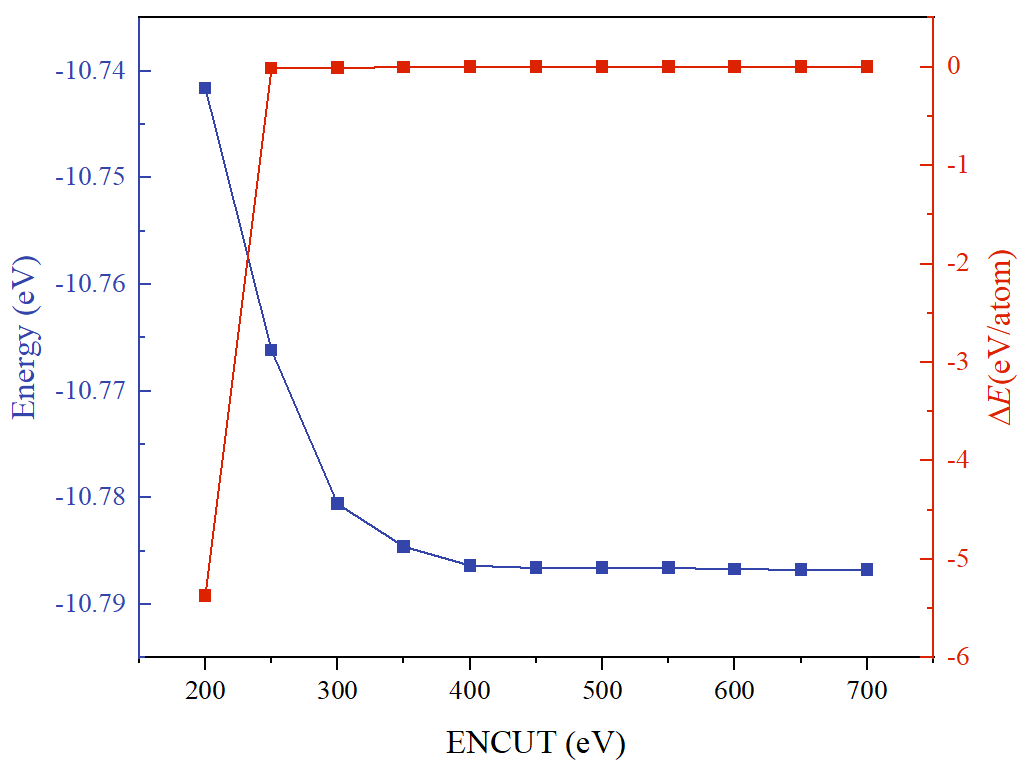
\includegraphics[width=1\linewidth]{VASP计算/静态自洽与电荷密度/能量计算/fig/截断能收敛性测试.png}
    \caption{截断能收敛性测试}
    \label{fig:能量计算-截断能收敛性测试}
\end{figure}

\begin{attention}
    在截断能的选择上,通常有一个理论最小值,也就是你所选择的赝势中\keywordin{POTCAR}{ENMAX}的最大值。设置的截断能必须比这个数值大才有可能保证准确性。例如,在本例中,如果查看我们使用的Si的赝势,里面有\code{ENMAX = 245.345},表明我们计算时所使用的截断能必须比这个数值大。通常情况下,使用\code{ENMAX}的1.3倍到1.5倍是合适的。
\end{attention}

\begin{extend}
    虽然我们多次说明:在计算时应当指定截断能,但事实上\code{ENCUT}本身是有默认值的,这个默认值就是赝势文件中\code{ENMAX}的最大值。尽管如此,对于不同的体系可能会有不同的默认值,在计算时为了统一,还是应当设置\code{ENCUT}。
\end{extend}

\subsubsection{K点测试}

关于K点的测试,方法与截断能完全类似,这里只给出最终结果如图\ref{fig:能量计算-K点收敛性测试}所示。可以发现,当K点取$9\times9\times9$时,体系能量收敛。

\begin{figure}
    \centering
    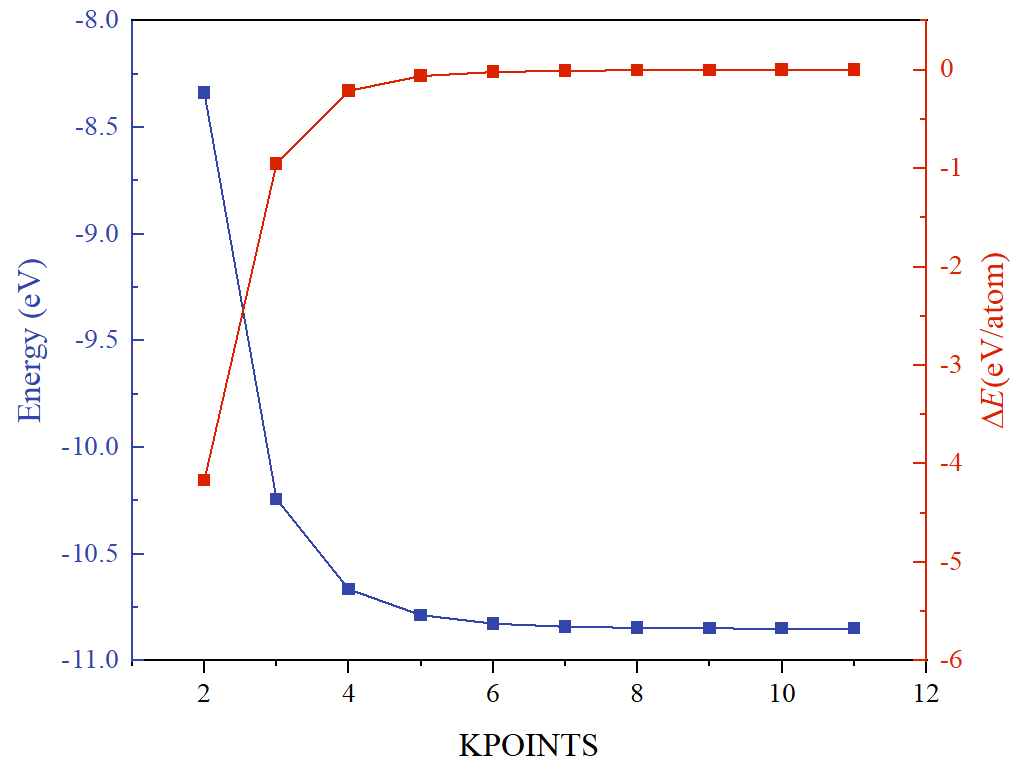
\includegraphics[width=1\linewidth]{VASP计算/静态自洽与电荷密度/能量计算/fig/K点收敛性测试.png}
    \caption{K点收敛性测试}
    \label{fig:能量计算-K点收敛性测试}
\end{figure}

\begin{attention}
    上述收敛性测试的例子仅是一个参考,实际情况还需要结合机时与计算时间综合考虑。此外,在这里我们所给出的结果是计算前用来做参数测试的步骤,在后续教程中,我们都不会进行这一步。其中有一些情况是结合经验选择的参数,有些是做过收敛性测试。在实际计算时,应结合实际情况选择参数。
\end{attention}

% \subsection{错误处理}\label{subsec:节标题-错误处理}
% % 请在本节列出可能遇见的错误与解决方法

% \subsubsection{错误1}

% \subsubsection{错误2}

% \subsubsection{错误3}
% 请在下方的大括号相应位置填写正确的节标题和标签,以及作者姓名
\section{磁矩计算}\label{sec:磁矩计算}
\sectionAuthor{Jiaqi Z.}

% 请在下方的item内填写本节知识点
\begin{Abstract}
    \item 知识点1
    \item 知识点2
    \item 知识点3
    \item 知识点4
    \item ...
\end{Abstract}

% 请在正文相应位置填写正确的小节标题(或小小节标题),同时将标签的“节标题”和“小节标题”改为实际内容

\subsection{小节标题}\label{subsec:节标题-小节标题}

\subsubsection{小小节标题}

\subsection{小节标题}\label{subsec:节标题-小节标题}


\subsection{错误处理}\label{subsec:节标题-错误处理}
% 请在本节列出可能遇见的错误与解决方法

\subsubsection{错误1}

\subsubsection{错误2}

\subsubsection{错误3}

% \input{VASP计算/写在前面/写在前面.tex}
% \input{VASP计算/电子性质/电子性质.tex}
\chapter{能带计算}\label{chap:能带计算}
\minitoc
\input{VASP计算/能带计算/能带基础理论/能带基础理论.tex}
\input{VASP计算/能带计算/VASP计算能带过程/VASP计算能带过程.tex}
\input{VASP计算/能带计算/能带绘图与后处理/能带绘图与后处理.tex}
% 请在下方的大括号相应位置填写正确的节标题和标签,以及作者姓名
\section{HSE能带计算}\label{sec:HSE能带计算}
\sectionAuthor{Jiaqi Z.}

% 请在下方的item内填写本节知识点
\begin{Abstract}
    \item 如何计算HSE能带
\end{Abstract}

% 请在正文相应位置填写正确的小节标题(或小小节标题),同时将标签的“节标题”和“小节标题”改为实际内容

在之前介绍PBE能带计算时提到,\emph{使用PBE计算会得到带隙偏小的情况},而这对于高精度计算显然是不合适的。因此,在大多数计算能带的论文中都需要其他泛函如HSE计算得到的能带。因此,在本节我们将讨论如何使用HSE计算能带并给出更加准确的带隙。

\subsection{结构优化与自洽计算}\label{subsec:HSE能带计算-结构优化与自洽计算}

在本节我们将讨论的结构是金刚石,其\code{POSCAR}文件如下所示:

\begin{lstlisting}[caption=POSCAR]
C2
1.0
        2.5269944668         0.0000000000         0.0000000000
        1.2634972334         2.1884414035         0.0000000000
        1.2634972334         0.7294804678         2.0632823422
    C
    2
Direct
        0.750000000         0.750000000         0.750000000
        0.500000000         0.500000000         0.500000000
\end{lstlisting}

对于HSE泛函计算能带,结构优化过程与前面\ref{subsec:VASP计算能带过程-结构优化}所介绍的步骤完全相同,因此这里不再赘述。

对于自洽计算,\code{KPOINTS}则需要使用hse的K点。生成方法可以使用\code{vaspkit-3-302/303}生成\code{KPATH.in}后使用\code{vaspkit-25-251}生成\code{KPOINTS},其中可以根据需要选择Monkhorst-Pack Scheme或Gamma Scheme方法生成K点\footnote{一般来说,使用Monkhorst-Pack生成K点精度较高,但对于六方晶系,则需要选择Gamma方法。}。然后需要依次输入scf所使用k点密度(通常设定为\code{0.04})以及计算能带所需要的k点密度(通常也设定为\code{0.04})

同时,在计算scf时还需要将\code{INCAR}的\code{LWAVE = .TRUE.}以生成波函数文件,以便计算能带时使用。下面是一个参考使用的\code{INCAR}文件:

\begin{lstlisting}[caption=INCAR]
Global Parameters
ISTART =  1
ISPIN  =  1
LREAL  = .FALSE.
ENCUT  =  600   
PREC   =  Accurate
LWAVE  = .TRUE.  
LCHARG = .FALSE.  
ADDGRID= .TRUE.

Static Calculation
ISMEAR =  0       
SIGMA  =  0.05    
LORBIT =  11      
NEDOS  =  2001    
NELM   =  60      
EDIFF  =  1E-08       
\end{lstlisting}

\subsection{HSE能带计算}\label{subsec:HSE能带计算-HSE能带计算}

上一步计算完成后,将\code{KPOINTS}, \code{POTCAR}, \code{POSCAR}和\code{WAVECAR}文件拷贝(或移动)至新的目录(暂且命名为\code{hse-band},使用\code{vaspkit-101-STH6}生成HSE计算的\code{INCAR}文件,调整必要的参数后如下所示:

\begin{lstlisting}[caption=INCAR]
Global Parameters
ISTART =  1
ISPIN  =  1
LREAL  = .FALSE.
ENCUT  =  600
PREC   =  Accurate
LWAVE  = .FALSE.
LCHARG = .FALSE.
ADDGRID= .TRUE.
    
Static Calculation
ISMEAR =  0
SIGMA  =  0.05
LORBIT =  11
NEDOS  =  2001
NELM   =  60
EDIFF  =  1E-08
    
HSE06 Calculation
LHFCALC= .TRUE.
AEXX   =  0.25
HFSCREEN= 0.2
ALGO   =  ALL
TIME   =  0.4
PRECFOCK= N
\end{lstlisting}

这里面的关键参数是\keyword{AEXX},表示杂化泛函所占的比重,通常设定为0.25是比较合适的。但\emph{这一比值会影响到带隙的大小},因此在必要的时候需要进行调整以适应实验结果。

将上述文件提交计算,由于HSE能带计算精度较高,因此需要时间较长\footnote{在测试计算时,64核计算时间为7.7个小时。}。

\subsection{HSE能带计算后处理}\label{subsec:HSE能带计算-HSE能带计算后处理}

与\ref{sec:能带绘图与后处理}一节所介绍的类似,在HSE计算后也需要对数据进行处理,绘图。但在一些细节上有些许不同:

\begin{itemize}
    \item 在绘制能带图之前,需要确保当前目录下有\code{KPATH.in}文件(可以直接使用\code{vaspkit-3-302/303}的方式生成,也可以直接从之前\code{scf}目录下复制过来;
    \item 使用\code{vaspkit-25-252}生成能带数据,所得到的\code{BAND.dat}和\code{KLINE.dat}文件可以将其放入Origin等软件中绘图(方法参考\ref{sec:能带绘图与后处理}一节,在此略)
\end{itemize}

生成能带数据后,可以通过\code{BAND\_GAP}文件查看计算得到的带隙。在本地测试时,得到结果为5.29 eV,与文献\footnote{Stoliaroff, A. \& Latouche, C. Accurate ab initio calculations on various PV-based materials: Which functional to be used? The Journal of Physical Chemistry C 124, 8467–8478 (2020).}结果5.38 eV接近。

同时,我们也可以利用\ref{sec:VASP计算能带过程}所介绍的PBE能带计算方法,对金刚石的PBE带隙进行计算。结果发现其带隙为4.12 eV,显然小于HSE带隙。

\chapter{态密度计算}\label{chap:态密度计算}
\minitoc
% 请在下方的大括号相应位置填写正确的节标题和标签,以及作者姓名
\section{态密度基础}\label{sec:态密度基础}
\sectionAuthor{Jiaqi Z.}

% 请在下方的item内填写本节知识点
\begin{Abstract}
    \item 态密度(DOS)的概念
    \item 分波态密度(PDOS)的概念
    \item DOS图与PDOS图的简要分析方法
\end{Abstract}

在本章我们将要讨论态密度(Density of State, DOS)的计算。从物理实质上来说,态密度和能带所包含的信息是大致相同的。例如,通过态密度和能带我们都可以知道材料带隙值的大小,判断导电性。但相比于能带,态密度还具有如下不同:

\begin{itemize}
    \item 对于超胞(通常还包括掺杂)等情况,能带结构会变得复杂,通常需要配合反折叠技术进行解释;而态密度对于超胞则是\emph{成比例缩放},因此会更加直观;
    \item 态密度相比于能带,可以计算分波态密度(Projected Density of State, PDOS)。利用PDOS,可以看到原子轨道(如O的2p轨道、Ti的3d轨道等)对态密度的贡献,从而可以进一步分析其物理机理;
    \item DOS图在绘制时忽略了波矢$k$信息,因此根据态密度无法分析带隙的类型是直接带隙或间接带隙。因此对于动量相关的信息,只能通过能带进行分析\footnote{进一步地,能带可以根据价带顶和导带底的能量对$k$的导数得到有效质量,DOS图就无法得到这一结论。}。
\end{itemize}

因此,在本章,我们将讨论如何使用VASP计算态密度,包括总态密度与分波态密度,还会包括考虑自旋极化的态密度绘制。

\subsection{态密度概念}\label{subsec:态密度基础-态密度概念}

我们并不会在这里详细说明态密度与能带的详细推导方法(可以参考相关的物理教材)。简单来说,在固体中由于电子的能级非常密集,为\emph{准连续分布},因此像原子那样标定每个能级是没有意义的。参考对应的概念,考虑能量在$E\sim E+\Delta E$之间的电子态数目,若电子态数目由为$\Delta Z$,则态密度定义为

\begin{equation*}
    N(E)=\lim\limits\frac{\Delta Z}{\Delta E}
\end{equation*}

对于已知能带而言,即已知$E(k)$关系,通过推导(参考黄昆著《固体物理学》)可以知道其态密度可以表示为

\begin{equation*}
    N(E)=\frac{V}{(2\pi)^3}\int\frac{\dd{S}}{\abs{\nabla_kE}}
\end{equation*}

除此之外,在考虑电子态的时候,如果仅考虑某个原子轨道的电子对能带的贡献,则所绘制的\emph{仅考虑对应轨道电子}的态密度称为\emph{投影态密度}(Projected Density of States, PDOS)。

\subsection{简要分析态密度和投影态密度}\label{subsec:态密度基础-简要分析态密度和投影态密度}

与能带类似,态密度也可以用来判断材料的带隙(但不能判断带隙类型为直接带隙还是间接带隙)。例如,在后面我们将会计算得到Si的态密度如图\ref{fig:态密度基础-Si态密度}所示。可以发现,Si的带隙大约为0.7 eV。

\begin{figure}
    \centering
    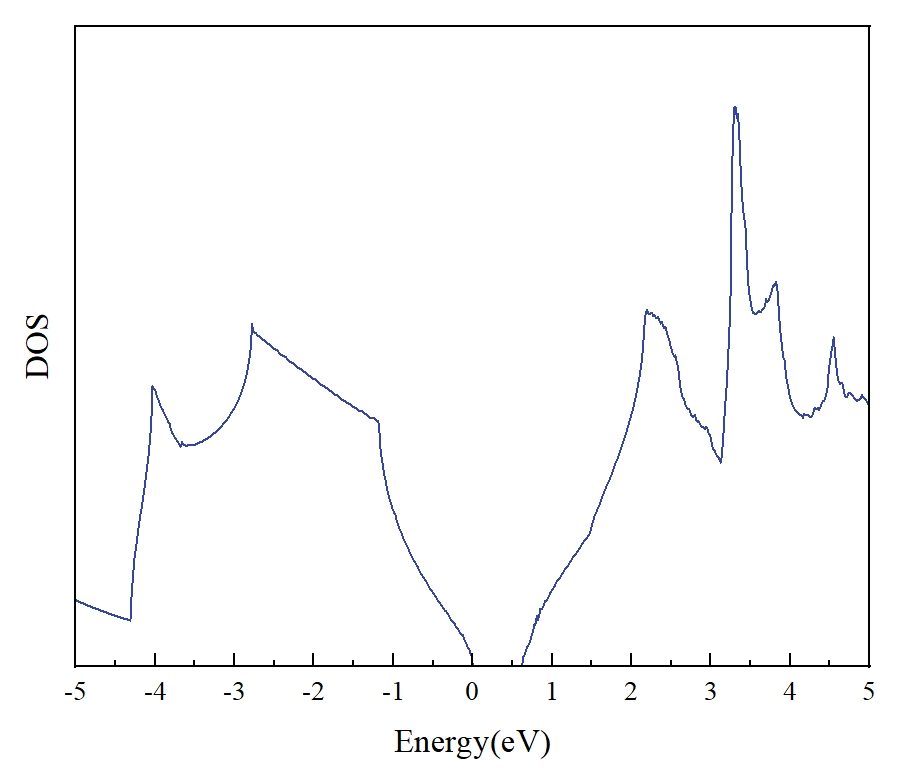
\includegraphics[width=1\linewidth]{VASP计算/态密度计算/态密度基础/fig/Si态密度.png}
    \caption{Si态密度}
    \label{fig:态密度基础-Si态密度}
\end{figure}

再比如,对于PDOS而言,我们可以通过态密度的重叠情况判断原子之间的杂化成键。例如,图\ref{fig:态密度基础-PDOS例子}中计算了Li吸附在不同\ch{TiS2}下的态密度,可以发现Li和Ti,Li和S之间存在着轨道重叠,表明两个原子的电子处在同一个电子态,即发生了\emph{轨道杂化}\footnote{参考文献:Tian, R. et al. Point defects-induced adsorption and diffusion of lithium on monolayer titanium disulfide: A first-principles study. Applied Surface Science 553, 149448 (2021).}。

\begin{figure}
    \centering
    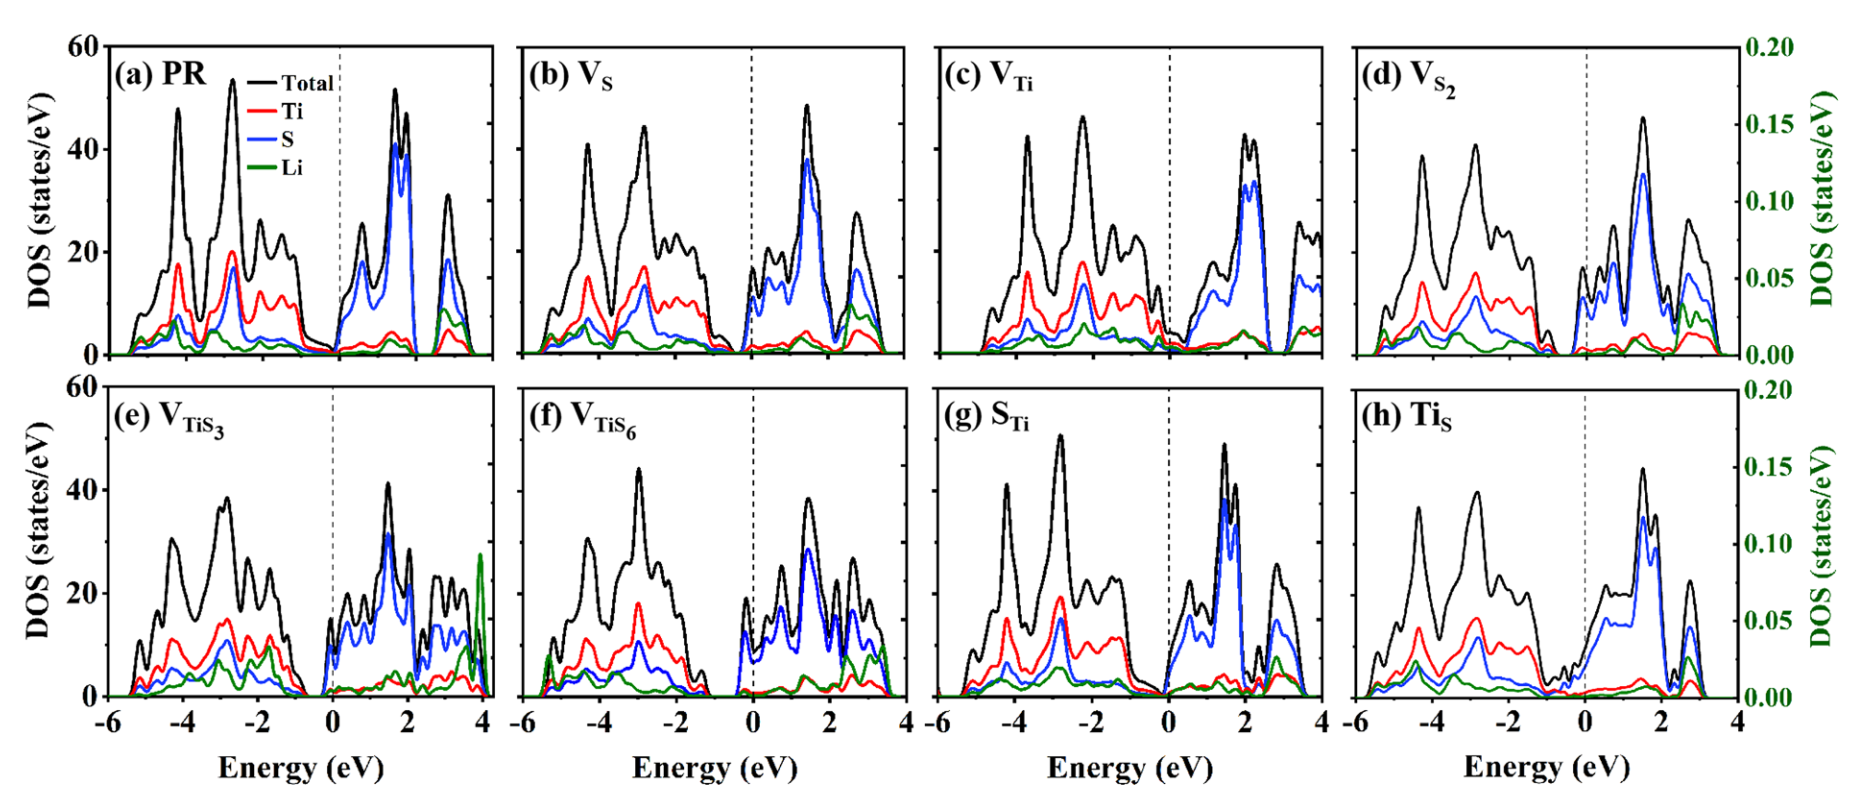
\includegraphics[width=1\linewidth]{VASP计算/态密度计算/态密度基础/fig/PDOS例子}
    \caption{PDOS例子}
    \label{fig:态密度基础-PDOS例子}
\end{figure}

% \subsubsection{小小节标题}

% \subsection{小节标题}\label{subsec:节标题-小节标题}


% \subsection{错误处理}\label{subsec:节标题-错误处理}
% % 请在本节列出可能遇见的错误与解决方法

% \subsubsection{错误1}

% \subsubsection{错误2}

% \subsubsection{错误3}
\input{VASP计算/声子谱计算/声子谱计算.tex}

    \part{Python与机器学习}

    \chapter*{Python与机器学习:前言}

这一部分是整套教程的最后一部分,主要介绍关于机器学习的相关算法和程序实现方法。目前,机器学习以及人工智能相关算法与技术正在爆发式涌现出来,大预言模型(LLM)频繁更新迭代,在科研领域使用人工智能的相关技术正逐渐成为科研领域的前沿方法。尤其是2024年诺贝尔物理学奖和化学奖分别颁发给与人工智能相关的技术,更是进一步促进了人工智能在科研领域的应用。

得益于Python语言强大的库函数支持,目前大多数机器学习算法都是基于Python语言实现。考虑到读者的编程水平不同,本部分的前两章将首先介绍关于Python语言的基本应用,分别针对Python的内置语法(如基本的数据结构、程序结构等)和频繁使用的库函数(如NumPy、Matplotlib等)进行讲解。

之后,我们将详细介绍大多数机器学习算法的原理和具体应用,由于计算性能的限制,考虑到机器学习算法在性能不是太好的电脑上也可以运行并得到理想结果,我们会花费较大的篇幅介绍机器学习的算法,包括它们的数学原理、程序实现和具体的应用方法。

对于有条件的情况下,我们将简单介绍关于神经网络(在有些地方可能也会将其称作“深度学习”)的一些算法与实现。对于有能力(特别是算力)的读者可以尝试了解并编写一些简单的程序来运行它们。考虑到大多数读者所使用设备的算力水平以及所使用的硬件,本教程在深度学习部分所使用的代码大多是基于英伟达Nvidia的常规显卡(如Nvidia GTX4060等显卡)实现并测试的。因此,我们并不会涉及太大与太复杂的神经网络。为了拓展大家的应用场景,我们在最后会讨论使用云端服务器的算力(考虑到像Colab等服务器对网络要求较高,且不稳定,我们在介绍云服务器时会使用百度飞桨的云服务器进行演示)运行神经网络的方法。

\section*{关于练习题与难度分类}

这一部分的很大内容是在介绍编程的,因此不做编程练习是不行的。同时,在介绍机器学习算法时,我们又不得不介绍很多的数学原理以及相应的概念,因此,也需要读者对其中一些数学原理有所了解。在每一节的结束时,我们都会尽量设置一些练习题,以便读者可以练习并检测自己编程能力的掌握情况。但不同的难度放在一起,对于初学者而言做困难的题目显然是有些不合适的。因此,我们希望参考《计算机程序设计艺术》这本书中对练习题的难度分类算法,简单将题目难度的“十位数”划分为以下几个类型:

\begin{itemize}
    \item 00: 这种题目通常都是非常简单的概念题,对于大多数读者而言,这类题目在几秒钟之内就可以思考出来(但需要你对本节内容有所掌握)
    \item 10: 这种题目可能需要你稍作思考,甚至可能在必要的地方需要你回去查阅相关的内容,但难度不会太大。对于编程题而言,这通常会是10行左右的程序,你可能在3-5分钟时间就可以思考出来并完成它们;
    \item 20: 这种题目的思考量会明显更大一点,可能需要你对前文内容有足够的理解。对于编程题而言,这可能需要你稍微思考一下算法(可能并不简单),并且程序量大约在20行-30行左右。你可能需要十几分钟乃至几十分钟左右来思考并完成它们;
    \item 30: 对于程序算法的思考量,或者运算会更多。在这时候你可能会需要编写一个比较完整的程序(或者算法)来实现一个具体的功能。程序量大约在50行左右,且所使用的算法更复杂。这种题目通常适合作为程序设计课程的课后作业,你所需要的时间大约以小时计;
    \item 40: 这种题目可能在编程上更适合作为课程设计。程序量大约在100行左右,且需要你对算法、程序语言有更深的理解,甚至需要你有一些创造性的想法在里面。通常来说,完成这个题目可能需要以天为单位;
    \item 50: 这种题目往往是很难实现的,或者这种题目绝不是可以凭一己之力完成的。对于一些特殊的内容(尤其是在机器学习部分),如果你有幸实现了这种算法,请务必分享给我们。我们会非常高兴看到这一进步。
\end{itemize}

在题目编号中,为将“编程题”和一般的概念题做区分,我们会使用“P”来表示编程题。同时,在机器学习部分,有些题目可能对于数学要求较高(可能使用了高等数学部分的内容),我们会使用“M”表示。

题目难度数值对5的余数表示所需要的时间量估计,对于再一步细分的难度,则在中间插值取得,将其划分为分度值为1的刻度。因此,对于难度为25和难度为24的题目,前者所需要的时间可能更少,但需要更多的思考量和创造性。

这里特别注意的一点是:对于出题的人来说,严格给出题目难度是非常困难的,而且所使用的程序行数也不是绝对的。因此,每个题目的难度仅是作为读者选择题目的参考(我们强烈建议读者完成难度在30以下的所有题目)。

\section*{关于这一部分的“错误处理”}

对于编程而言,我们所说的“错误”可以包括两种类型——一种是编程语言语法上的错误,另一种是算法上的错误。在每一节的后面,我们会尽可能给出代表性的编程时所可能发生的错误,这些错误很多都是“致命性”的,即程序语言会中断执行的错误(在后面我们会了解到,这种东西叫做“异常”)。这些错误在很多时候是可以避免的。

而对于算法上的错误,我们确实很难避免,而且这些错误难以排查。它们在程序编写过程中,可能是一个符号输入错误,或者变量赋值错误等。这些错误导致程序在程序层面是正确执行了,但没有得到预期的结果。这一部分错误我们只能尽可能在正文中进行“启发”,从而帮助读者理解算法设计时需要注意的一些事项。对于笔误等原因所发生的错误,我们“心有余而力不足”。

\section*{练习题}

\begin{itemize}
    \item [00] 这一部分我们所需要学习的编程语言是什么?
    \item [M14] 对于函数$f(x)=x\sin(2x)$,求它的导函数$f_x(x)$
    \item [P50] 编写一个大预言模型(LLM),帮助你回答上面的问题。
\end{itemize}


\chapter{基础Python语法}\label{chap:基础Python语法}
\minitoc
% 请在下方的大括号相应位置填写正确的节标题和标签,以及作者姓名
\section{安装Python}\label{sec:安装Python}
\sectionAuthor{Jiaqi Z.}

% 请在下方的item内填写本节知识点
\begin{Abstract}
    \item 什么是Python程序语言
    \item 如何安装Python IDLE
    \item 如何安装Anaconda
\end{Abstract}

在本章,我们将讨论Python程序语言的基本语法(所谓基本语法,指的是Python程序语言本身所提供的编程语法,不包括后面所使用的库函数)。这一部分对于整个Python语言是基础,因此有必要仔细学习并掌握它们。

但在开始之前,让我们先来介绍一下Python语言。

Python由荷兰国家数学与计算机科学研究中心的Guido van Rossum(吉多·范罗苏姆)于1990年代初设计,作为一门叫做ABC语言的替代品。 

\begin{extend}
    ABC语言是Guido参加设计的一种教学语言,可以说是专门针对非专业程序员设计的。但是,ABC语言并没有成功,究其原因,Guido本人认为是由于其非开放造成的。因此,他本人决心在Python语言中避免这一错误。

    可以说,Python语言是从ABC语言发展而来,并结合了如Shell语言和C语言的习惯。
\end{extend}

Python语言目前已经称为最受欢迎的程序语言之一,在2019年1月,TIOBE编程语言排行榜将Python语言评为2018年度语言。由于Python语言的简洁性、易读性和可扩展性,在国外大多数科研机构都逐渐开始使用Python语言进行科学计算研究,同时,像麻省理工学院的计算机科学与编程导论课也使用Python语言讲授。同时,Python大量的科学计算扩展库也帮助科研人员使用(其中最著名的就是NumPy、Pandas和Matplotlib,分别用来进行数组矩阵处理,数值运算和绘图,在后面的章节我们也会介绍着三个库)。

Python语言具有如下特点:

\begin{itemize}
    \item 简单易学:Python语言极其容易上手,且接近自然语言;
    \item 免费、开源:Python语言是自由软件之一,你可以很容易下载到对应的源代码,并对其进行修改,并用于新的软件中;
    \item 高级语言:相较于C语言,Python语言没有指针等类似的概念,你不需要管理内存分配等底层细节;
    \item 可移植性:目前,Python语言已经被移植到如Linux、Windows、Mac OS操作系统中。在运行时,你不需要编译成二进制代码,而是直接从源代码中运行\footnote{从底层来看,Python实际上是将程序翻译成字节码(byte code),再使用如Python Virtual Machine(Python虚拟机)来执行这些字节码。这类似于Java语言的运行方式,但Python的虚拟机相较于操作系统本身更远,抽象程度更高。};
    \item 可扩展性:Python语言可以支持部分程序使用C/C++语言编写,然后提供对应的接口,从而在Python中调用C/C++语言;反之也可以(将Python语言用于C/C++语言中),这可以使得程序更加容易移植,且效率更高;
    \item 丰富库:Python提供了大量的标准库,包括正则表达式、文档处理、数据库、网页、GUI图形界面等。除此之外,还有许多第三方库,如前面所提到的科学计算所使用的NumPy、Matplotlib,以及机器学习会用到的Scikit-learn、TensorFlow等,都可以方便在Python中调用。
\end{itemize}

\subsection{如何安装Python}\label{subsec:安装Python-如何安装Python}

我们将介绍两种Python的安装——一种是最简单的Python本身安装(它也提供了一种最简单的IDLE编辑器),另一种是Anaconda。对于初学者,或者简单使用的读者而言,可以考虑第一种安装(它更简单);但我们强烈建议安装Anaconda,相比于前者,它集成了更多的软件包,可以适用于更复杂的项目,而且也方便后续不同库和软件版本的管理。

\subsubsection{直接安装Python}

\begin{attention}
    在编写这一节时,Python的最新版本是3.13. 根据大版本号分类,可以将Python分为Python2和Python3版本。在本章所使用的Python版本为Python3.11.5,你可以根据需要选择安装合适的版本。

    通常来说,Python3内部的版本没有明显的语法差异(对于一般使用者而言无需深入关心),如果你是为复现文献或使用别人的代码而下载Python,可能会看到有使用Python2的。但是,Python官方已于2020年停止对Python2版本的更新,因此,除非是迫不得已的理由,否则你没有任何理由使用Python2版本。

    我们将在后面的教程中说明Python2和Python3的区别。
\end{attention}

直接安装Python可以到官网:https://www.python.org/downloads/ 下载对应的版本。在官网找到对应的版本后,点击右侧的“Download”,在下方选择对应的版本(以本地为例,使用Windows Installer (64-bit)作为安装版本)

\begin{extend}
    在安装时可能会注意到,对于64位系统分为普通的“64-bit”和“ARM64”版本。前者实际上就是我们大多数人所熟知的x64架构(又名AMD64或Intel64架构),是由AMD公司提出并迅速被Intel公司采用的一种指令集扩展(前身是x86架构,也就是我们所熟悉的32-bit操作系统),主要通过提供复杂的指令集减少编译器工作量,但同时需要消耗更多的资源。

    后者(ARM64)是由ARM Holdings设计的用于ARM的v8-A的架构,在设计时考虑更小的指令集从而使得能耗更低,常用于移动设备和嵌入式系统中。目前,也有处理器使用ARM64架构,例如苹果公司于2020年推出的Apple M1处理器就是采用的ARM64架构。
\end{extend}

下载完成后,双击打开安装包如图\ref{fig:安装Python-Python-IDLE安装}所示。\emph{将下方的Add Python.exe to PATH勾选},然后选择Install Now即可默认安装。安装完成后在开始菜单可以找到Python对应版本,在cmd命令行输入\code{python --version}也可以输出对应的版本号(表明安装成功)。

\begin{figure}
    \centering
    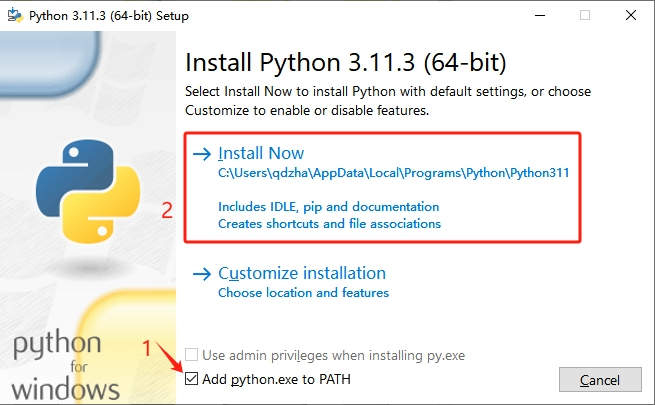
\includegraphics[width=1\linewidth]{Python与机器学习/基础Python语法/安装Python/fig/Python-IDLE安装.png}
    \caption{Python-IDLE安装}
    \label{fig:安装Python-Python-IDLE安装}
\end{figure}

\subsubsection{使用Anaconda安装Python}

相比于前面直接安装Python,安装Anaconda更有助于后续的学习。因此我们建议读者(尤其是面向科研的工作人员)安装Anaconda。

在安装Anaconda时,可以前往Anaconda的官网\footnote{https://www.anaconda.com/download},在网页中可能会需要提供邮箱,但提供与否并不影响实际下载。我们可以选择下方的“skip registration”进入下载页面。选择对应的操作系统版本点击下载即可。

\begin{attention}
    这里面的版本可能会与需要使用的版本不同,将在后面介绍如何在Anaconda中使用特定的Python版本(创建虚拟环境)。在这里不必担心所下载具体Python版本。
\end{attention}

下载完成后打开安装程序,如同正常的安装过程默认安装即可,在勾选选项时(如图\ref{fig:安装Python-Anaconda安装}所示)建议选择与图示相同的选项,点击“Install”安装即可。安装完成后可以在开始菜单找到“Anaconda”目录,打开其中的“Anaconda Prompt”,输入\code{python --version},若出现正常的版本号,则表明安装成功。

\begin{figure}
    \centering
    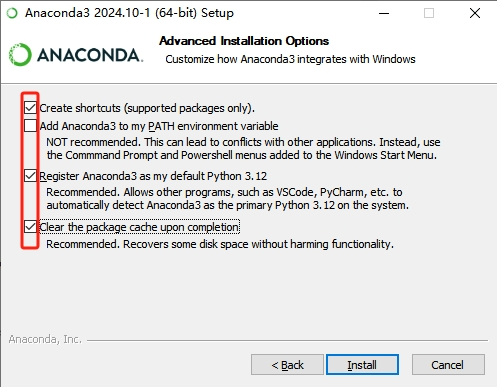
\includegraphics[width=1\linewidth]{Python与机器学习/基础Python语法/安装Python/fig/Anaconda安装.png}
    \caption{Anaconda安装}
    \label{fig:安装Python-Anaconda安装}
\end{figure}

\begin{extend}
    正如前面所说,在安装Anaconda时我们没有指定具体的Python版本,而在使用Anaconda时,可以通过创建虚拟环境指定代码运行时所使用的版本。具体创建方法为:

    \begin{enumerate}
        \item 在“Anaconda Prompt”中使用命令\code{conda create -n [环境名] python=[版本号]}创建对应的版本环境,例如,以3.11为例,使用\\\code{conda create -n py311 python=3.11},完成后输入“y”安装对应包即可下载对应版本的Python;
        \item 完成后输入\code{conda activate [环境名]}即可激活刚才所创建的环境。例如,以刚才所创建的环境为例,输入\code{conda activate py311}即可切换至环境中。切换后在命令行前面应当会有以括号开头的环境名表示当前环境;
        \item 在当前环境下输入\code{python --version}查看对应安装版本。
    \end{enumerate}
\end{extend}

\subsection{运行第一个Python程序}\label{subsec:安装Python-运行第一个Python程序}

下面,我们将测试自己所下载的Python是否可用,一个最简单也“约定俗成”的一段代码是“Hello World!”程序,即\emph{尝试输出“Hello World!”字符串}。针对上述两种安装方法,我们可以有不同的运行方式:

\subsubsection{使用命令行模式}

对于直接安装Python的用户而言,可以在开始菜单找到Python的IDLE,这是一个简单的集成开发环境。当你打开时,可以看到如图\ref{fig:安装Python-IDLE窗口}所示的IDLE窗口,前面的\code{>>>}表示等待输入命令。对于输出Hello World,可以执行下面的命令:

\code{print("Hello World!")}

输入后点击回车,在下方应当输出了“Hello World!”,从而表明Python安装正确。

\begin{figure}
    \centering
    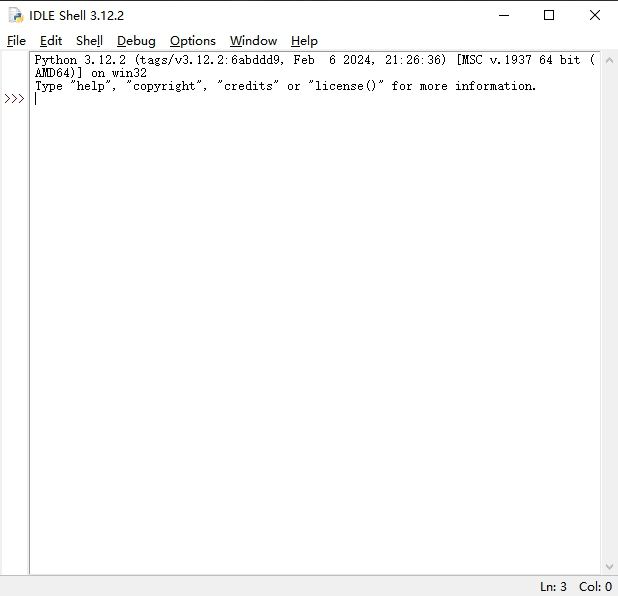
\includegraphics[width=1\linewidth]{Python与机器学习/基础Python语法/安装Python/fig/IDLE窗口.png}
    \caption{IDLE窗口}
    \label{fig:安装Python-IDLE窗口}
\end{figure}

\begin{attention}
    与其他编程语言类似,在编写Python程序时,请务必确保你的符号(引号内的文字可以除外)都是\emph{英文半角符号}。
\end{attention}

如果使用的Anaconda,则在打开Anaconda Prompt并激活环境后,输入\code{python}也可进入类似于上方IDLE的环境,可以执行正常的命令编写。与上面的步骤类似,可以执行\code{print("Hello World!")}查看输出结果

\begin{attention}
    在Anaconda Prompt当中,如果要退出Python则可以输入\code{exit()}或\code{quit()}退出至普通命令行模式。
\end{attention}

\subsubsection{使用文件模式}

上面的命令行只能适用于比较简单的命令测试,对于后面我们所学习的编程,大多数情况下是需要编写Python文件的。Python语言程序文件的后缀名是\code{*.py}。对于使用IDLE的用户,可以使用菜单栏的“File”-“New File”\footnote{或者使用快捷键Ctrl+N}创建一个文本文件。之后的编程则是在这个文本文件中进行。

以“Hello World!”为例,编写下面的文件并保存为\code{hello.py}文件

\begin{lstlisting}[language=python,numbers=left,caption={hello.py}]
print("Hello World!")
\end{lstlisting}

保存后点击上方的“Run”-“Run Module”(或者使用快捷键F5),则可以在前面的IDLE窗口中看到如下输出:

% \begin{lstlisting}
% =================== RESTART: C:/Users/qdzha/Desktop/hello.py ===================
% Hello World!
% \end{lstlisting}

\begin{lstlisting}
====== RESTART: C:/Users/qdzha/Desktop/hello.py ======
Hello World!
\end{lstlisting}

其中,第一行表示运行的程序路径与文件名,后面则是正常的程序执行过程(在这里输出“Hello World!”)

如果你使用的是Anaconda Prompt,则可以在外面使用文本编辑器(如记事本等)输入上面的程序并保存为\code{hello.py}(注意修改后缀名),然后再Anaconda Prompt的对应环境中输入命令:\code{python [程序路径名]}即可运行。

\begin{extend}
    虽然我们没有详细介绍关于Windows操作系统下的命令行操作,但在第一部分的\ref{subsec:通配符-使用通配符进行文件目录操作}一节中我们稍微提到了关于cmd的一些命令。与Linux类似,在使用Anaconda Prompt进行目录与文件操作时,在目录相关操作中(打开目录、切换上一级目录)与Linux系统的命令完全相同。

    因此,你可以在Anaconda Prompt当中使用\code{cd}命令打开至你所保存程序的目录。但是需要注意的是,由于Windows操作系统中硬盘分区的问题,当你希望切换至其他盘符时(例如,从C盘切换至D盘),则直接输入\code{d:}即可。在切换盘符后再切换回来时会保留你上一次的目录。

    在执行\code{python [程序路径名]}时,这个路径名可以是绝对路径(从盘符开始算起),也可以是相对路径名(从当前命令行所在目录开始算起)
\end{extend}

\subsubsection{*使用Anaconda Spyder编辑器}

这一部分是针对于Anaconda用户的,主要是为了方便文本编辑和程序运行测试。Spyder是一个使用Python语言的跨平台的科学运算集成开发环境,相比于其他编辑器,Spyder在调试代码时包含一个“工作空间”,方便对变量的值进行调试(类似于MATLAB)。

但在使用Spyder之前,我们需要做一点准备工作:首先,如果你使用的是自己创建的环境,在激活环境后\emph{需要安装spyder包},在Anaconda中,安装Spyder包的方法是在当前环境下输入\code{conda install spyder},搜索完必要包后输入“y”安装。

安装完成后在开始菜单打开Spyder(Anaconda目录下),找到对应的Spyder(一般括号后有对应的环境名)打开,即可进入界面如图\ref{fig:安装Python-Spyder界面}所示。类似于MATLAB界面,在右上角可以选择文件目录,点击上方菜单栏“文件”-“新建文件”可以创建Python程序。输入上面的Hello.py程序并保存即可创建文件。

\begin{figure}
    \centering
    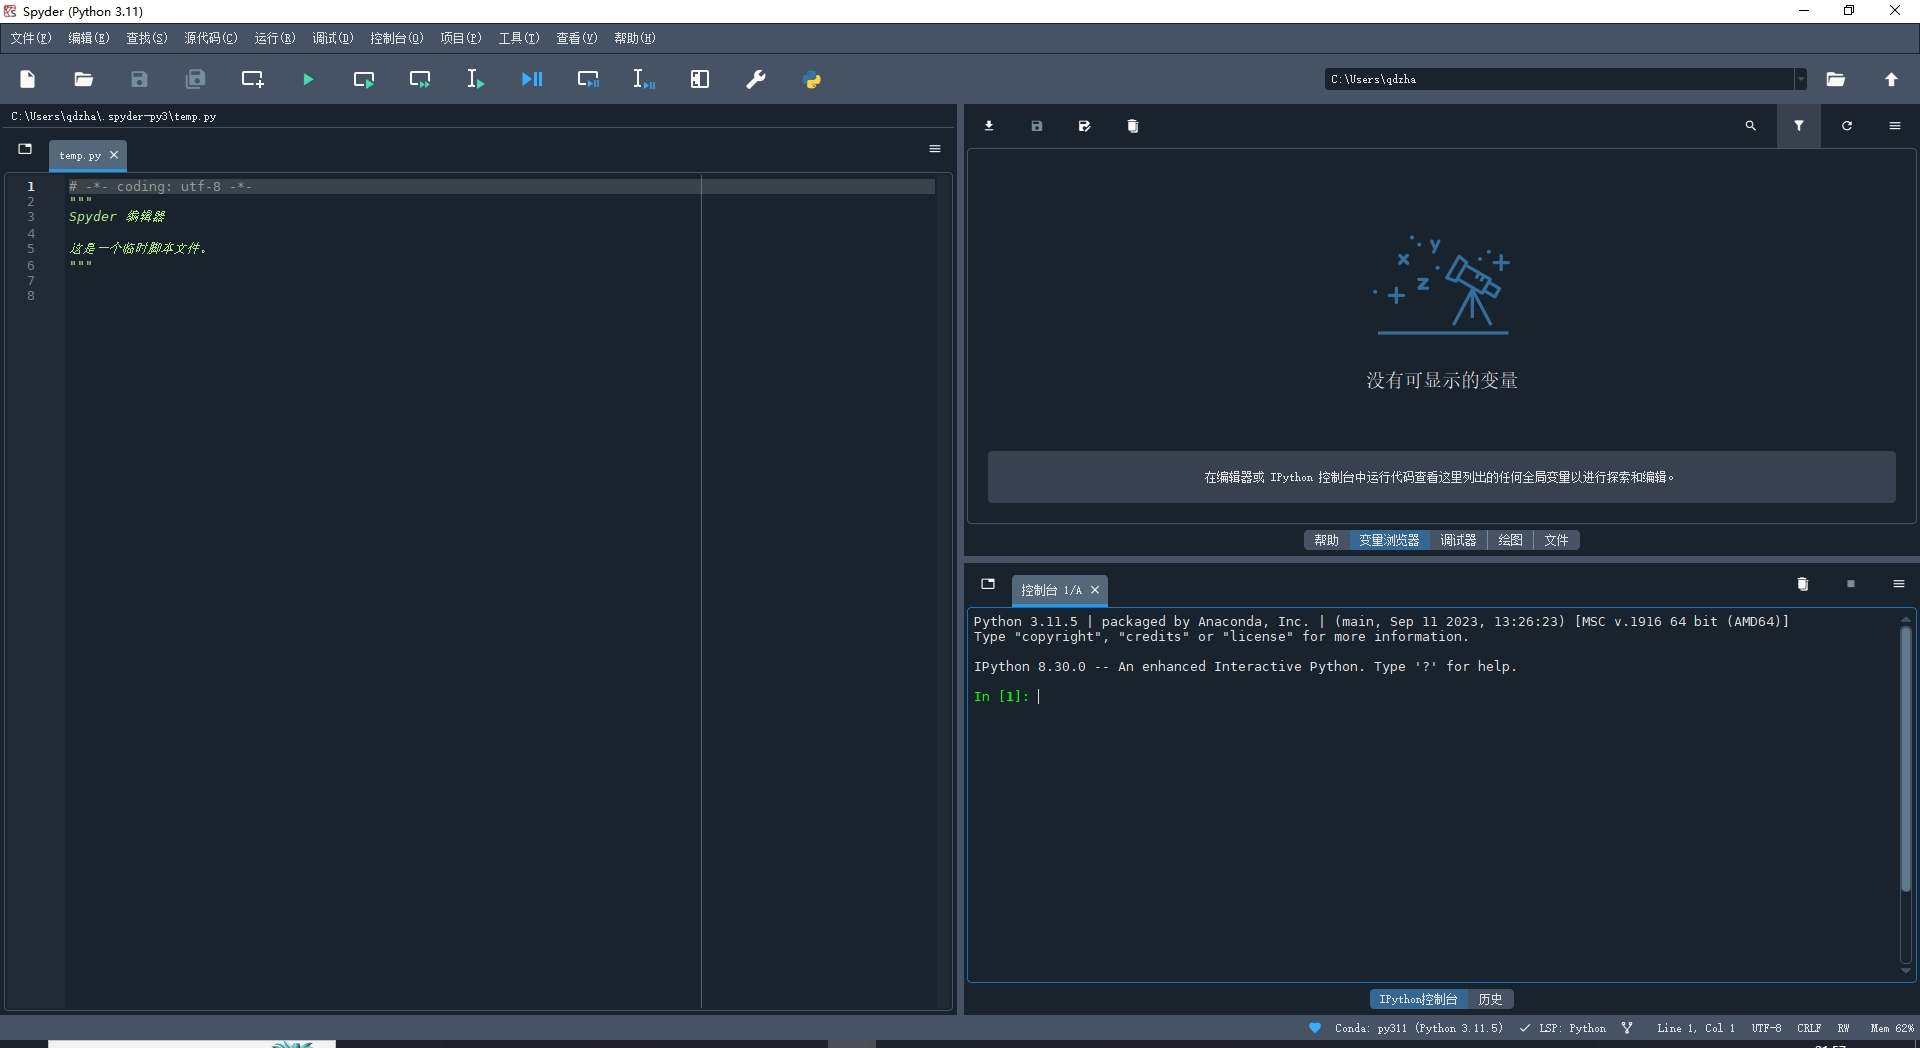
\includegraphics[width=1\linewidth]{Python与机器学习/基础Python语法/安装Python/fig/Spyder界面.png}
    \caption{Spyder界面}
    \label{fig:安装Python-Spyder界面}
\end{figure}

运行文件时,可以点击上方的“运行文件”图标,或使用快捷键F5,即可在右侧控制台看见对应的输出。

\begin{extend}
    除此之外,你也可以使用Anaconda Navigator工具来管理环境与使用Spyder。这个工具是使用窗口的方式进行操作,因此更加人性化。在开始菜单打开Anaconda Navigator后,如图\ref{fig:安装Python-Anaconda Navigator界面}所示,点击上方的下拉选项,选择需要切换的环境,找到Spyder启动即可(如果没有安装对应的包则会提醒“Install”安装。

    \begin{figure}
        \centering
        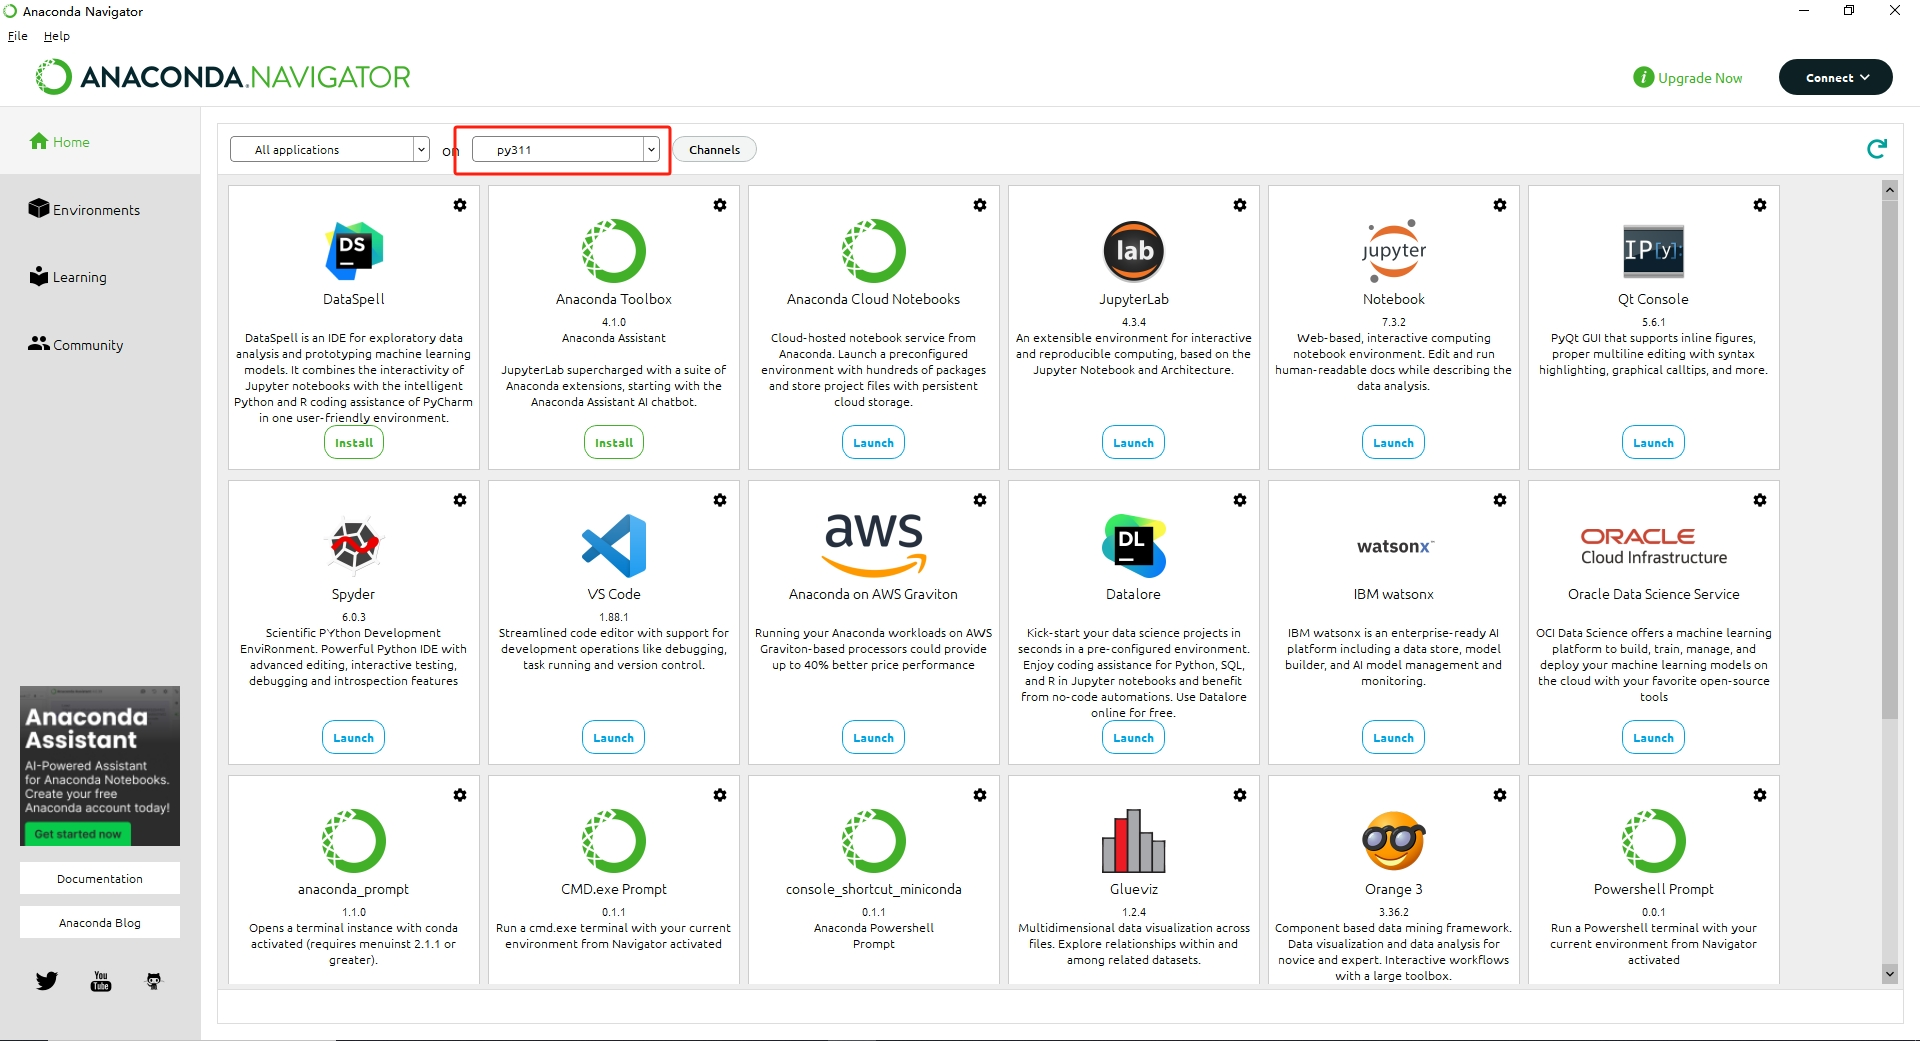
\includegraphics[width=1\linewidth]{Python与机器学习/基础Python语法/安装Python/fig/Anaconda Navigator界面.png}
        \caption{Anaconda Navigator界面}
        \label{fig:安装Python-Anaconda Navigator界面}
    \end{figure}

    在第二章以及后面的章节中可能会使用到另外的工具——Jupyter Notebook(或者Jupyter Lab),你也可以使用这种方式来安装并执行(相比于安装Jupyter内核,这种方式更加容易上手),在后面的章节我们将不会介绍如何在对应环境下启动Jupyter Notebook。
\end{extend}



\subsection{练习题}\label{subsec:安装Python-练习题}

\begin{itemize}
    \item [01] Python语言所使用的文件后缀名是什么?
    \item [02] 本节介绍了哪两种运行Python程序的方式?各有什么优劣?
    \item [10] 如果需要使用Anaconda创建一个名字叫“Exercise”的虚拟环境,Python版本为3.12,应当如何创建?
    \item [21] 在Anaconda中,可以使用\code{conda env list}查看所创建的虚拟环境及其对应的目录。尝试使用对应的目录,在cmd模式下使用对应的虚拟环境,并执行前面所编写的程序。
    [提示:不同的环境目录下都有一个\code{python.exe}文件,与cmd执行Python程序时的命令\code{python}是一样的]
    \item [P03] 仿照正文中的程序,编写一个Python程序,输出“Hello Python”。
    \item [P25] 在Python2和Python3当中,一个最大的区别是输出的方式不一样。对于Python3(前文所介绍的)是使用\code{print()}函数输出,输出内容作为函数的参数(在后面的章节中我们会详细介绍函数);而对Python2而言,使用的是\code{print}语句,即\code{print [字符串]}的方式。请使用Anaconda创建一个Python2.7的虚拟环境(尽管现在不建议),重写上面的“hello.py”程序,使其在Python2.7版本下可以正常输出“Hello World!”
    \item [16] 如果你下载使用的是Python IDLE,在下载时曾设置“Add Python.exe to PATH”。事实上这个PATH在Windows操作系统中可以通过右键单击“此电脑”-“属性”-“高级系统设置”-“环境变量”查看。请尝试查找对应的目录在哪里?如果删除掉这个环境变量会发生什么?
    \item [P18] 对于课题组内的服务器而言,有些服务器已经配置了Python或者Anaconda,请尝试在Linux服务器中编写正文中所提到的“Hello World!”程序。
    [提示:你可以通过\code{python --version}输出版本号的方式检查是否安装并可以正常调用Python。]
\end{itemize}

\subsection{错误处理}\label{subsec:安装Python-错误处理}

\subsubsection{SyntaxError: invalid character}

这种错误可能是由于你错误使用了符号字符,例如,当你在输入括号时使用中文括号,则会触发这个错误。因此,\emph{在编写程序时,除引号内,不要使用中文输入法}。

    \backmatter

    \printindex

    \bibliography{reference}

\end{document}